%% ----------------------------------------------------------------
%% Thesis.tex -- MAIN FILE (the one that you compile with LaTeX)
%% ---------------------------------------------------------------- 

% Set up the document
\documentclass[a4paper, 11pt, oneside]{thesis}  % Use the "Thesis" style, based on the ECS Thesis style by Steve Gunn

\usepackage{verbatim}

% Include any extra LaTeX packages required
\usepackage[square, numbers, comma, sort&compress]{natbib}  % Use the "Natbib" style for the references in the Bibliography

\usepackage[nottoc]{tocbibind} % bind bibliography to the table of contents
\usepackage{verbatim}  % Needed for the "comment" environment to make LaTeX comments
\usepackage{vector}  % Allows "\bvec{}" and "\buvec{}" for "blackboard" style bold vectors in maths
\usepackage[table]{xcolor}
\usepackage{minted}
\usepackage{hyperref}
\usepackage{placeins}

\hypersetup{urlcolor=black, colorlinks=true}  % Colours hyperlinks in black, can be distracting if there are many links and colored blue.

%% ----------------------------------------------------------------

\begin{document}
\frontmatter      % Begin Roman style (i, ii, iii, iv...) page numbering

% Set up the Title Page
\title  {Automated Stress Testing of Websockets in a Microservice Environment}
\authors  {David Ahern}
            
\addresses  {\groupname\\\deptname\\\univname}  % Do not change this here, instead these must be set in the "Thesis.cls" file, please look through it instead
\date       {\today}
\subject    {}
\keywords   {}

\maketitle
%% ----------------------------------------------------------------

\setstretch{1.3}  % It is better to have smaller font and larger line spacing than the other way round

% Define the page headers using the FancyHdr package and set up for one-sided printing
\fancyhead{}  % Clears all page headers and footers
\rhead{\thepage}  % Sets the right side header to show the page number
\lhead{}  % Clears the left side page header

\pagestyle{fancy}  % Finally, use the "fancy" page style to implement the FancyHdr headers
%% ----------------------------------------------------------------
% Declaration Page required for the Thesis, your institution may give you a different text to place here


\Declaration{

\addtocontents{toc}{\vspace{1em}}  % Add a gap in the Contents, for aesthetics

I, David Ahern , declare that this proposal titled, `Automated stress testing of web sockets in a microservice environment' and the work presented in it are my own. I confirm that:

\begin{itemize} 
\item[\tiny{$\blacksquare$}] This work was done wholly or mainly while in candidature for an masters degree at Cork Institute of Technology.
 
\item[\tiny{$\blacksquare$}] Where I have consulted the published work of others, this is always clearly attributed.
 
\item[\tiny{$\blacksquare$}] Where I have quoted from the work of others, the source is always given. With the exception of such quotations, this project report is entirely my own work.
 
\item[\tiny{$\blacksquare$}] I have acknowledged all main sources of help.
 
\item[\tiny{$\blacksquare$}] I understand that my project documentation may be stored in the library at CIT, and may be referenced by others in the future.
\\
\end{itemize}
 
 
Signed:\\
\rule[1em]{25em}{0.5pt}  % This prints a line for the signature
 
Date:\\
\rule[1em]{25em}{0.5pt}  % This prints a line to write the date
}
\clearpage  % Declaration ended, now start a new page

%% ----------------------------------------------------------------
\begin{comment}
% The Abstract Page
\addtotoc{Abstract}  % Add the "Abstract" page entry to the Contents
\abstract{
\addtocontents{toc}{\vspace{1em}}  % Add a gap in the Contents, for aesthetics

The Thesis Abstract is written here (and usually kept to just this page). The page is kept centered vertically so can expand into the blank space above the title too\ldots

}

\clearpage  % Abstract ended, start a new page
%% ----------------------------------------------------------------
\end{comment}
\setstretch{1.3}  % Reset the line-spacing to 1.3 for body text (if it has changed)

% The Acknowledgements page, for thanking everyone
\acknowledgements{
\addtocontents{toc}{\vspace{1em}}  % Add a gap in the Contents, for aesthetics

I would like to thank Dr Ruairi O Reilly for his advice, encouragement, expertise and continuous support. I would also like to thank my employers at Dell EMC for providing hardware necessary for conducting experimentation.

Lastly, I would like to thank my family and partner for their continued support throughout the research.

}
\clearpage  % End of the Acknowledgements
%% ----------------------------------------------------------------
\begin{comment}

\pagestyle{fancy}  %The page style headers have been "empty" all this time, now use the "fancy" headers as defined before to bring them back


%% ----------------------------------------------------------------
\lhead{\emph{Contents}}  % Set the left side page header to "Contents"
\tableofcontents  % Write out the Table of Contents

%% ----------------------------------------------------------------
\lhead{\emph{List of Figures}}  % Set the left side page header to "List if Figures"
\listoffigures  % Write out the List of Figures

%% ----------------------------------------------------------------
\lhead{\emph{List of Tables}}  % Set the left side page header to "List of Tables"
\listoftables  % Write out the List of Tables

%% ----------------------------------------------------------------
\setstretch{1.5}  % Set the line spacing to 1.5, this makes the following tables easier to read
\clearpage  % Start a new page
\lhead{\emph{Abbreviations}}  % Set the left side page header to "Abbreviations"
\listofsymbols{ll}  % Include a list of Abbreviations (a table of two columns)
{
% \textbf{Acronym} & \textbf{W}hat (it) \textbf{S}tands \textbf{F}or \\
\textbf{LAH} & \textbf{L}ist \textbf{A}bbreviations \textbf{H}ere \\

}

%% ----------------------------------------------------------------
% End of the pre-able, contents and lists of things
% Begin the Dedication page

\setstretch{1.3}  % Return the line spacing back to 1.3

\pagestyle{empty}  % Page style needs to be empty for this page
\dedicatory{For/Dedicated to/To my\ldots}

\addtocontents{toc}{\vspace{2em}}  % Add a gap in the Contents, for aesthetics

%%
\end{comment}
\mainmatter	  % Begin normal, numeric (1,2,3...) page numbering
\pagestyle{fancy}  % Return the page headers back to the "fancy" style

\begin{abstract}

Microservice architectures have seen widespread adoption in industry in recent years \cite{fowlerOnMicroservices}. They enable the separation of critical components into loosely coupled services, this, in turn, enables teams to adopt agile methodologies such as DevOps, continuous delivery, and test-driven development for validation.

A lesser used form of validating microservices is stress testing, which tests the robustness and error handling of systems under heavy load. Stress testing is often an afterthought until it becomes a critical issue. A reason this can be unappealing for teams to implement is due to the complexities required to set up a test infrastructure as well as the financial cost of hardware and test planning when compared to unit testing or integration testing.

This project demonstrates an approach to stress testing that validates and monitors services within microservice architectures by actively monitoring the underlying services of an application while testing is in progress, to allow developers gain a greater understanding of how increased traffic is affecting their systems. This framework currently stress tests web socket protocols, however, in the future this can be expanded for testing other protocols.

\end{abstract} % Abstract

\tableofcontents
\listoffigures

\chapter{Introduction}
\lhead{\emph{Introduction}}

Microservice architectures have been widely adopted over the past decade. Monolithic architectures require all code to be compiled into one single artifact. In contrast, applications built using a microservice architecture decompose the key parts of monolithic applications into smaller independent services. 

Microservice architectures are easier to scale than their monolithic counterparts. If developers detect that a service is under heavy load they can add more instances of that particular service, this is known as horizontal scaling. For a monolithic application to scale a developer would have to add more instances of the entire application, this is known as vertical scaling. 

Monolithic architectures are usually written in one programming language, this can be problematic as there is no one language that is suitable for every use case. Once developers have committed to using one language it is very hard to back out and use another language should requirements change. With microservices, developers have more freedom, if requirements change they can easily add new services written in a different language, and because services can be very small in size it is not uncommon to re-write services from scratch using a new language that makes sense to the new requirements.

In terms of agility microservices are widely accepted to be more in line with agile practices than monolithic architectures. This is due to the high degree of decoupling between services. In many companies there may be a single team assigned to one service.

Microservices do have some disadvantages. In larger applications there may be hundreds of services running. This makes automated monitoring of services very difficult when compared to monolithic applications which require monitoring a single service. A similar problem arises for debugging of applications. In a monolithic architecture a developer only needs to view a single log file file, however in a microservice architecture they will need to view log files coming from many services. 

Traffic monitoring is another problem for microservices. An example of this would be in a web application. If a user connects to our web interface, they may make a network request to login to the application. The network request may come into the microservice system and be forwarded on to any number of services before responding to a users request. Tracing the flow of network requests through the system and seeing how each service along the way is affected is important to maintaining a healthy, scalable system. 

Test driven development (TDD) in microservice architectures is a good way to try and circumvent some of these problems. By utilizing TDD, developers have re-assurance that what they are releasing to production environments is in working order. TDD comes in a variety of forms, such as unit, integration and end-to-end testing. There is also another form of testing known as stress testing which is the focus of this paper. 

Stress testing involves simulating a number of users to see if a system can handle certain loads. This is an important metric for developers. Without this testing in place, developers have no re-assurance that the system they are building can handle the number of users they are expecting. Without stress testing, it is highly likely that system will experience outages, which can lead to financial loss.

There are many tools available for stress testing applications. Apache JMeter is one such tool. These tools offer the ability to simulate many users. They can summarize the limits of an application such as how many requests made successful connections and how many requests failed. While this is useful it does not give any insights into how services within a microservice architecture have reacted to the test. We feel that a tool that could do both stress testing and can also give insights into how microservices react to tests would give developers a much better understanding of their design as well as making debugging a simpler process.

As part of this research paper we have developed a tool which can stress test websockets deployed in a microservice environment which can also monitor services individually within a microservice system. Throughout this paper we will summarize the main parts of this tool, how it was built and present our final results.

\section{Motivation}

To the best of our knowledge their are no tools on the market, that can combine both stress testing and monitoring of a microservice environment. The main beneficiaries of this tool are developers utilizing websockets who wish to gain deeper insights into how large user bases will affect their systems. As more companies adopt agile methodologies such as continuous delivery, there is a greater need to actively test their software before it reaches production to prevent any degradation in performance.

The second motivation of building this tool is to easily allow developers adopt stress testing tools. Testing methods such as unit tests and integration tests are widely used, however in many cases stress testing is often seen as an after thought. In our experience this has held true, and is only considered when the worst case scenario occurs and production environments are down for hours or days leading to financial loss.

\section{Research Questions and Objectives}

\subsection{Research Question}

With the ever growing importance of websockets in a microservice environment as will be described in Chapter 2. We believe it is important to actively stress test these websocket implementations. The aim of this project is to create a websocket stress testing tool that can also monitor microservice environments and each of the underlying services in order to give developers a greater understanding of how large amounts of traffic can affect their environments.

\subsection{Research Objectives}

\begin{itemize}
  \item To develop a websocket stress testing tool that can also monitor microservice environments.
  \item Summarize results of a test to a developer using an intuitive interface.
  \item Test the system using a variety of WebSocket server implementations. Using GoLang and NodeJS to see how scalable the platform is.
  \item To integrate the platform with existing continuous integration tools.
\end{itemize}

\subsection{Structure of this document}

Chapter 1 describes the overall objects of this research thesis while introducing microservices and how many companies are adopting this architecture over monolithic architectures. Chapter 2 will detail the background research into the various technologies that will be utilized for building this system. This will mainly detail microservices and websockets and how they have evolved over time. Chapter 3 will describe how the stress testing tool was put together, detailing the technologies used and the motivation behind each chosen technology. Chapter 4 will detail the results of developing the stress testing tool as well as giving a comparison of each of the various websocket implementation's between different languages. Chapter 5 will discuss the conclusions and finding of this research as well as detailing future work. % Introduction

\chapter{Background}
\lhead{\emph{Background}}

In this chapter, background research will be presented. This includes an overview of the current technologies in the area as well as the technologies used in this project and a review of the current research.

\section{Test Automation}

One of the goals of automated testing is to reduce the number of manual test cases. It is important to note that automated testing does not completely remove the need for manual testing, instead it will free testers from repeating tedious tests, and allow them to focus on exploratory testing. Automated testing comes in many forms, such as Unit or Integration testing. There are also many agile methodologies around testing. So-called extreme programming allows for a number of practices around automated testing. For example, developers are encouraged to pair on many tasks. This involves both developers sitting in front of 2 screens which show the same code. This is important as with pairing it is important not to sit in unnatural positions as pairing can take place over a number of hours, and developer health should be taken into consideration. During pairing, developers can write tests as they are developing software. One method called ping pong pairing involves one developer writing a failing unit test, the next developer will then make the failing test pass. Then the roles are reversed. This gives both developers a chance at writing both tests and implementations, increasing both of their knowledge of the code base. 

One paradigm which is often used to describe what test automation is the testing pyramid which is depicted in figure \ref{fig:testing-pyramid}

\begin{figure}[!h]
  \centering
    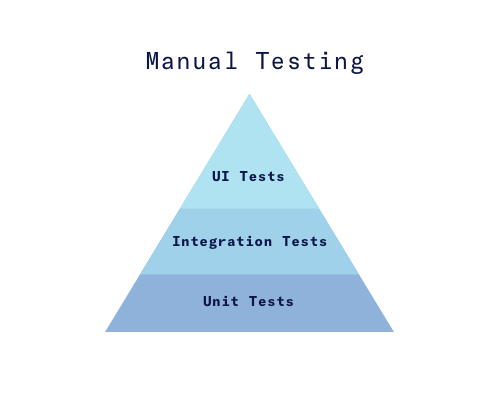
\includegraphics[width=0.8\textwidth]{figures/testing-pyramid.png}
    \caption{Testing pyramid}
    \label{fig:testing-pyramid}
\end{figure}

The testing pyramid states that tests on the bottom are fast running such as unit tests. They are relatively inexpensive to write. As we move up the pyramid we see that tests are much slower to run and become more expensive in terms of time to run and infrastructure required.

\section{Stress Testing}

Stress testing involves the process of simulating multiple users against an environment to see can that environment handle a specified load. It is not clear where stress testing fits into the testing pyramid depicted in figure \ref{fig:testing-pyramid}. There are many stress testing tools on the market such as Apache JMeter, WebLOAD and LoadNinja. These tools fit will into integration environments. For example, when a developer pushes code changes to a code revision tool such as Git, a continuous integration tool such as Jenkins can run a build which stress tests the changes using JMeter, if any of the code changes cause degradation then JMeter will pick this up and possibly fail a build, meaning that the developer must fix the issue before they are allowed to merge their changes to a master branch. This prevents any performance degradations reaching production.

\section{Websockets}

Websockets are a TCP based protocol\cite{8089962}. There have been a number of patterns and methods used in the past to simulate real-time communication. These include both polling and long polling. With polling, a client would make a request to a server continuously every few seconds. This method of communication had some drawbacks. It required connections to make a TCP handshake every time it reconnected. This handshake is costly as it takes a number of milliseconds to initiate. This is not a huge deal with just one connection. However when this is scaled up to hundreds of thousands of users then this TCP handshake will really impact a system\cite{5735801}. HTTP handshakes involve sending an SYN packet to the server which responds with an SYN-ACK to acknowledge the request then the client sends another SYN packet and connection is then established\ref{fig:http-handshake}\cite{5735801}. HTTP(s) further complicates the process as now the communication takes place over TLS (Transport Layer Security)\ref{fig:https-handshake}. 

\begin{figure}[ht]
  \centering
    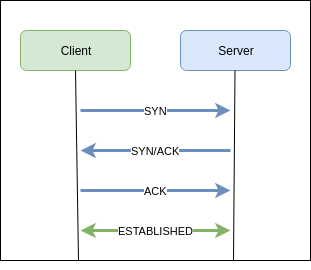
\includegraphics[width=0.5\textwidth]{figures/http-handshake.png}
    \caption{HTTP handshake}
    \label{fig:http-handshake}
\end{figure}

\begin{figure}[ht]
  \centering
    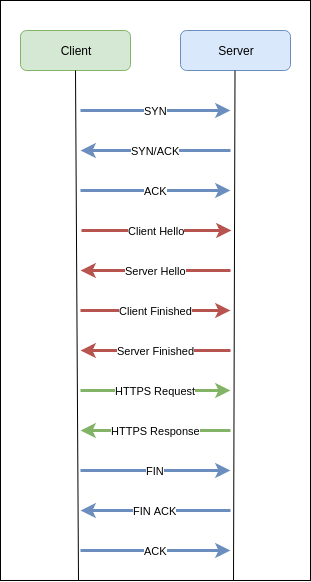
\includegraphics[width=0.5\textwidth]{figures/https-handshake.png}
    \caption{HTTP(s) handshake over TLS}
    \label{fig:https-handshake}
\end{figure}

Long polling tries to address this issue by making a request from the client to the server. The server then keeps the connection open for a specified amount of time. The server will wait for new information to arrive from somewhere. If data arrives before the connection times out then the connection is immediately terminated and the data is sent to the client. If no data has arrived by the time the connection times out then the connection is terminated and no data is sent to the client. In both cases, the client will then reconnect and wait for more data to arrive. As specified in \cite{6364271}, long polling has one drawback in real-time communication systems in that it needs more than one connection to achieve bi-directional communication.

There has been a huge shift from desktop devices to mobile devices\cite{6365155}. It has been proven that communication methods such as polling and long polling can have a negative effect on the battery life of mobile devices\cite{6364271}. This is due to the continuous connection and re-connection cycles, which are further exasperated by the fact that most of these connections are over cellular networks.

WebSockets aim to try and fix a lot of these shortcomings. This includes the ability to have full-duplex communication over a single persisted connection. WebSocket support is available in all major browsers, including mobile browsers. Once a connection is established between a server and a client, then both can communicate freely with each other by sending data encapsulated within a frame plus 2 extra bytes of payload, which is a huge reduction in payload from HTTP requests. There are 2 main stages of establishing and sending data over web sockets. These include the handshake stage, which like polling and long polling is done over HTTP. The reason this is done over HTTP is that web socket protocols are built on top of HTTP. They also had backward compatibility in mind with HTTP in that you can send a GET request to a web socket server and the server will send back an UPGRADE request telling the client that communication over a web socket protocol is available. The client can then decide whether to upgrade or not.

\subsection{Resource Usage}

Websockets have been proven to require fewer system resources for real-time communication than polling and long polling. A study which done a comparative analysis of AJAX polling versus web sockets found that polling increases the memory consumption over time compared to web sockets which maintained a fairly constant memory consumption throughout\cite{6601579}. In terms of bandwidth usage when comparing polling versus web sockets it was concluded that polling uses a larger amount of bandwidth over time, the reason for this was that polling required 256 bytes of extra data to be sent over the wire even if that 256 bytes of data is not used up, this means that in some cases there is can be a lot of white space sent over the network. The second reason was that the header data required for polling is significantly larger than that of a web sockets header\cite{6601579}.

\subsection{Keep Alive Mechanisms}

Because WebSocket servers can hold potentially hundreds of thousands of connection open simultaneously, it is reasonable that the server may want to recycle some of these connections to prevent itself from becoming overloaded. Websockets support a keep-alive mechanism to tell the server that the client is still actively using the connection. This is done in the form of a PING/PONG request. The server will send a ping request to the client, if the client is still active then it will respond with a pong. If the client does not respond then the server is free to terminate the connection and free up some resources in the process. 

\subsection{Websockets in a microservices environment}

Microservice architectures compliment web sockets in a number of ways. In front of most microservice environments is an API gateway\cite{6885428}. This is a reverse proxy between a companies API layer and the end user. It acts as a security barrier preventing the user from having direct access to any of the underlying API's. Nginx is an example of a reverse proxy with web socket support. When a web socket connection is created Nginx will stream the web socket request onto the target service, the data will flow from the service through the gateway to the user's client. 

While microservices do well to compliment web sockets, sadly there are cases where a microservice can be difficult for web sockets. Scaling applications is one such situation. Scaling means having multiple instances of the same service running at the same time with a load balancer in front which can choose the healthiest instance of a service to route requests to. Load balancing web sockets can be a tricky task depending on how the web socket server is set up. The issue is that when you connect to a service, that connection is long-lived if there is a drop in connection and the web socket server re-connects then it is possible that the new connection may be connected to a different instance of the server the web socket was previously connected to. For this reason, it is a good practice to make web socket servers stateless. Best practices suggest connecting the service to a backend queue such as RabbitMQ, Apache Kafka or Redis. This way of a web socket connection is dropped it will matter less which instance the reconnection request connects to.


\section{Monitoring}

As mentioned briefly in Chapter 1 monitoring of microservices can be a difficult task. This is due to the distributed nature of microservices. Monitoring can take many forms, such as resource monitoring or usage monitoring or log monitoring. with resource monitoring, we are trying to track the amount of CPU and memory usage or number of disk input/output jobs over a period of time. This is a powerful metric if utilized correctly. Companies such as Netflix and Facebook, use a method known as AB testing. With AB testing we can introduce new services that are meant to replace an existing service. For example, if there is a service that recommends shows to watch, which is a service Netflix provides. If developers want to rewrite this service in a new language, they can do this and then deploy the new service side by side with the existing service. The new service would accept the same inputs as the existing service however the outputs would only be persisted from the existing service. The developers can then monitor resources over a period of time, if they see that the new service is using fewer resources than the existing service, this can be used as evidence to determine that the new service is a suitable replacement.

Usage monitoring, on the other hand, may involve tracking the number of users that visit our services. In the case of a web application, this can be the number of users that have visited our website. To get the most out of this most monitoring tools allow the ability to break the visitor usage down into what routes they have visited. For example, if we have a route in our web application that is for listing friends of a user, we could track if this route is being used or not. This type of tracking is very valuable as it can be used to determine if the features of an application are providing value to a user. NewRelic is a tool which provides this service as a cloud offering. With NewRelic, developers need to install an agent into their code. This agent will then communicate with the NewRelic service and store usage statistics. 

Log monitoring in microservices is difficult. As mentioned in Chapter 1 this is again due to the distributed nature of microservices. Developers are no longer dealing with one single log, they are instead dealing with a log from each connected service in the system. With larger environments, debugging systems can prove a laborious task. One common way that companies use to provide an easier debugging experience is to use a central log aggregator. With this, all logs from each of the services are forwarded to the central log service. One of the most common platforms for log aggregation is the ELK stack. which is short for Elasticsearch, Logstash, and Kibana. These are 3 individual open source tools, however, they can be combined to make a powerful log aggregation tool. ElasticSearch is a distributed search and analytics engine, it can be used to index any form of data for later searching. Logstash is a lightweight data processing pipeline tool that can accept data from a number of sources and finally Kibana lets developers visualize search queries in elastic search and provides a powerful user interface. With the ELK stack in place, developers can search for keywords such as "ERROR" or "CRASH" that occurred in logs in a specific time frame, making debugging systems less monotonous. Logz.io is an example of a company who has taken this one step further. They have combined machine learning that can scan and make sense of each log input. Their system can actively inform developers of anything it finds in their logs that it has marked as interesting or potentially fatal. This reduces the workload of developers while debugging systems.

\section{Docker}

Docker is a tool that allows developers to create, deploy and run applications which are distributed as containers. Docker is often compared to virtualization tools such as Virtualbox and VMWare Fusion. We believe this comparison to be incorrect, the key difference being that virtualized run on top of a hypervisor which is running on top of a guest operating system, the running virtual machine has its own operating system such as Linux or Windows with its own memory management system. It is also possible to have multiple virtual machines running at the same time on a single machine. In comparison docker containers do not use a hypervisor, they are instead executed using the docker engine. Containers are considerably smaller and use fewer resources than virtual machines as well as having much faster startup times. Because of this docker containers are starting to be used for tasks such as integration testing.

Without docker, there was no real way to test an applications integration with a database such as MySql. When developers wrote tests they usually used an in-memory database such as H2. For example, if we are building a web application that has a rest endpoint for creating a shopping list we could write an integration test that would start the application and make a HTTP request to this endpoint and check if the endpoint stores our shopping list correctly. As the application is starting it would also start the in-memory H2 database. If the test passes we have some assurance that when our application reaches a production environment that it will just work. However, in reality, this is not always the case. In memory databases like H2 are not 100\% compatible with MySql, that being, some queries that work on H2 will not work on MySql and vice versa. Docker, on the other hand, allows developers to start a real MySql server within a Docker container for the duration of the integration test. Once the test completes the container is thrown away, ensuring that new tests will be using a completely fresh database. There are a number of libraries available that make starting and stopping of containers easy, such as \href{https://www.testcontainers.org/}{TestContainers} for Java and NodeJs.

\section{Kubernetes}

While docker can be useful for testing it is also a production-ready tool and works well in a microservice architecture. Docker Swarm and Kubernetes are the two main docker container orchestration tools on the market today. Docker Swarm was originally developed by docker themselves. This allows docker containers to be spread over a number of virtual or real machines, while docker swarm would handle all network activity between each of the containers by utilizing its own DNS server. Kubernetes was originally designed by Google, the project was originally called Borg while later changing to be called Kubernetes. Kubernetes was made open source by Google in 2014. It has many of the same features that docker swarm has including network and DNS. Kubernetes is also available as a cloud offering from GKE (Google Kubernetes Engine). 

Both Docker Swarm and Kubernetes allow defining microservices or infrastructure as code. For example, if we are building a microservices, we can define each of these microservices and the networking between them as code. This code can then be distributed to allow for repeatable environments. In the case of docker swarm, this code is defined in a file called docker-compose.yml. For Kubernetes there is a package manager called Helm which uses YAML files to orchestrate the environment.

\section{Cloud Foundry}

Cloud Foundry is a popular PaaS (Platform as a Service) system maintained by Pivotal Labs. One of its main goals is to make working with microservices easy for developers. Cloud Foundry uses a different container technology than we see in Kubernetes, instead of Docker it uses Droplets. Droplets allow users to specify run time environments known as buildpacks. For example, if we are building a NodeJS application we would use the NodeJS buildpack and if we were building a Java application we would use the Java buildpack. Droplets can then use the specified buildpack to provide a sandboxed environment to run an application. Resource limits can also be put on each running application, these include CPU, Memory, and Storage.

Cloud Foundry also supports the auto-scaling of applications. A developer can set thresholds on the amount of memory or CPU usage if this threshold is reached then the Cloud Foundry system will deploy another droplet alongside the existing droplets. In front of each droplet is a load balancer. The load balancer will route requests to each of the running instances of the applications in a round robin fashion.

Third party services such as MySql, Postgres, and MongoDB can be bound to applications. When binding services to an application the credentials of the service and connection URI will automatically be exposed to a running application in the form of environment variables. The application can then read these environment variables to connect to the service.

Cloud Foundry exposes a powerful rest API which can be used to query running applications and get usage statistics such as Memory CPU and storage of each running instance of an application. With this API it is also possible to get information on application states. As will be explained in Chapter 3 we will be utilizing this API to monitor running applications while we perform stress testing.

\section{Current State of the Art}

Automated testing has been utilized to great effect over the past 10 years due to the widespread adoption of agile methodologies. The journey from being a company not practicing agile to a company that does practice agile is a difficult one. Lawrence and YSlas suggested that cultural differences may play a part in this \cite{1667587}. Vriens and Barto suggested that senior management are often a roadblock in this transition, stating ``If this involvement by senior management results in micromanagement, the engineers will lose energy and self-direction resulting in an initiative-lacking organization`` \cite{4599511}. However, a successful transition will result in a highly collaborative and adaptive team free from the shackles of process.

Adopting a DevOps culture is key to being a successful agile practicing organization. One of the goals of DevOps is to bring software updates to production as quickly and as regularly as possible. To achieve this, organizations have to employ a high degree of automated testing. A study, conducted in 2019 concluded that performance evaluation of software was rarely used. The study found that only one-third of companies involved conducted performance evaluations on their systems. And 50\% of those who do performance evaluations spend only 5\% of their time working on these tests \cite{bezemer2019performance}. The study also presents a potential reason for this, stating that ``DevOps movement is
still in its infancy, and developers are still getting used to the opportunities that this movement offers in terms of automation of
performance engineering processes``.

Bezemer also suggests that the complexity involved in performance testing may act as a barrier for widespread adoption, and also concludes that current performance testing tools do not integrate well with current continuous integration tools such as Jenkins or TeamCity.

In our experience working in the software industry, these conclusions are accurate and from what we have seen, other forms of testing often take priority over performance testing. This can also be verified when looking at previous papers written on the subject. Weyuker states that often the primary issues that are reported from production environments are related performance degradation's when companies look into the reasons why this is the case, they usually find that there was no real test strategy for validating the performance of the application \cite{888628}.  % Background

\chapter{Solution Design and Implementation}

This chapter describes the architecture that was designed for this project. In the first part of this chapter, we will discuss each of the individual parts of the overall functioning stress test platform.In the later stages of this chapter, we will present some of the more relevant code snippets that make up the system and discuss how test-driven development helped us achieve the goal of creating this platform. Throughout this chapter you will see the term ws-flare used, this is because We have given the platform the name ws-flare which is short for WebSocket flare.

\section{Problem Definition}

This project aims to develop a tool for stress testing application which can easily integrate into continuous integration environments. The tool that we have created abstracts away the complexities of stress testing, such as automatically scaling using Kubernetes, as well as automatic monitoring of applications in a microservice environment, ensuring that developers have better insights into how their applications handle an abundance of users. Throughout this chapter, we will present the main technologies that we used while developing this tool.

\section{Technologies}

For this project, we have utilized the following technologies extensively.

\begin{itemize}
  \item NodeJS (Loopback 4)
  \item Angular
  \item Highcharts
  \item Docker
  \item Kubernetes
  \item MySQL
  \item RabbitMQ
  \item GraphQL
\end{itemize}

\subsection{NodeJS (Loopback 4)}

NodeJS was chosen for this project because of our own particular expertise with NodeJS. We were also concerned with using high memory consumption languages such as Java in this project as we would be running this application on a Kubernetes cluster. The main financial costs when it comes to Kubernetes or any cloud offering is memory and CPU usage. The more resources that are in use, the more the cost of running the platform will be. NodeJS, on the other hand, is much more lightweight. We found that 30 Megabytes of memory is more than enough to run a single microservice in this platform. 

We are also using a web framework called Loopback 4. This framework is written in typescript and has inbuilt support for test-driven development.

\subsection{Angular}

Angular is a popular open source, single page application framework developed and maintained by Google. We use this framework extensively for building the user interface of the ws-flare framework. Angular is written in typescript and comes with a powerful testing framework called TestBed which makes developing in a test-driven manner simpler.

\subsection{Highcharts}

In the ws-flare user interface, we display many graphs for showing the results of test jobs. Highcharts is a charting library, developed by HighSoft. It is free to use for open source applications and supports an abundance of graph types.

\subsection{Docker}

Each service in the ws-flare framework is built to run in a docker container. This is necessary as the framework is built to run on a Kubernetes cluster which needs docker in order to function. Each service is also deployed to Docker hub, which makes it easy for any company to import the framework into their environments.

\subsection{Kubernetes}

The ws-flare framework is built exclusively to run on Kubernetes clusters. This helps with scalability issues when simulating many thousands of connections as Kubernetes can run over many machines simultaneously. We also use Kubernetes package manager called helm. With helm we can easily distribute the framework and companies can install it into their own infrastructure.

\subsection{MySql}

We use MySql as the main data persistence database within the ws-flare framework. Data includes web socket metadata such as successful, failed and dropped connections as well as data gathered during monitoring of cloud foundry services. We run MySQL in high availability mode. For this, we have two instances of MySql running at the same time. One instance is for reads and the other instance is for writes. The reason for this is there are a lot of writes occurring during test runs. For example, while simulating 30000 connections, it is necessary to persist data for each connection in a short timeframe. While this is happening, users need to use the user interface to view test runs in real time. When users view the interface they are mostly reading information from the database. High availability prevents any latency when viewing the user interface.

\subsection{RabbitMQ}

Ws-flare is built using a distributed microservices architecture. Some services within the framework need to be able to talk to each other. RabbitMQ is a messaging queue which makes this possible. Services are able to listen to topics in RabbitMQ and other services can send messages to the topics. Once a service detects that a message has been sent they can then react to that service. Message queues are often considered as fire and forget mechanisms for sending messages. A service sends a message and does not care what will react to that message. This ensures that services are highly decoupled.

\subsection{GraphQL}

GraphQL is a new technology developed by FaceBook. It is built as an alternative to REST and is suited to largely decoupled microservices. In the ws-flare user interface, we query a lot of information to display results to a developer. With REST it would be necessary to send a request to each of the relevant services on the backend and aggregate the results on the user interface. With GraphQL however the user interface needs to send a query to one single service, and that service will aggregate the data coming from the other services. This makes working with many microservices much easier.

\section{Architecture}

There are a few terms going forward that need to be defined. Below is an explanation of these terms

\begin{itemize}
  \item \emph{Pod} Is a group of one or more docker containers with shared storage and network running within Kubernetes.
  \item \emph{JWT} stands for JSON Web Token is an open standard \href{https://tools.ietf.org/html/rfc7519}{RFC 7519} for securely transmitting data between 2 places in JSON format. For the purposes of this project, we will be using it for user authentication.
\end{itemize}

\begin{figure}[!h]
  \centering
    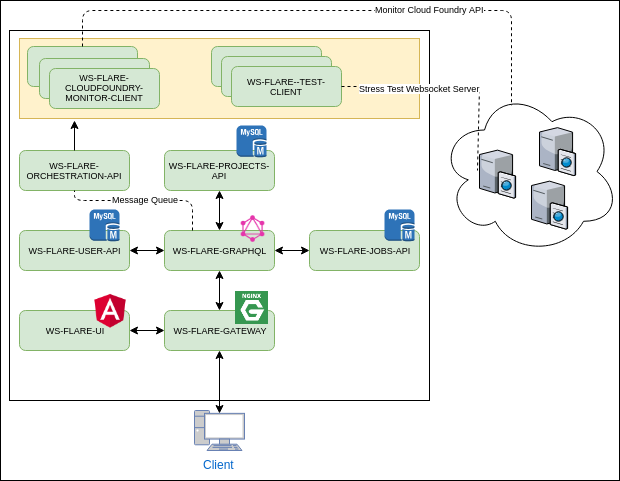
\includegraphics[width=0.8\textwidth]{figures/architecture.png}
    \caption{Architecture of the ws-flare platform}
    \label{fig:https-handshake}
\end{figure}

The project has been split up into a number of microservices to allow for maximum code readability and testability. The following microservices have been developed to make up the system.

\begin{itemize}
  \item ws-flare-ui
  \item ws-flare-user-api
  \item ws-flare-projects-api
  \item ws-flare-jobs-api
  \item ws-flare-orchestation-api
  \item ws-flare-cloud-foundry-monitor-api
  \item ws-flare-test-client
  \item ws-flare-cloudfoundry-monitor-client
  \item ws-flare-graphql
  \item ws-flare-gateway
  \item ws-flare-helm-chart
\end{itemize}

\subsection{ws-flare-ui}

This service is written in Angula7. It holds all the code for displaying the user interface to a user. We also use Highcharts as a charting library for displaying results.

\subsection{ws-flare-user-api}

Holds all user authentication information, such as email, user-name, and passwords. For making authentication requests we are using JWT tokens to allow a user to query the system. Without this security, any user could utilize the system to attack websites so it is important that we have this layer of security.

\subsection{ws-flare-projects-api}

The system allows users to create projects to logically separate each task. This is more for user convenience and adds to the overall UX aesthetics's of the system. All project and task information are stored within this service. 

\subsection{ws-flare-jobs-api}

This service holds information about currently running jobs. The system allows for running multiple jobs at the same time to allow to be truly embedded into continuous integration environments. This service is using MySQL for persisted storage. 

\subsection{ws-flare-orchestation-api}

This service handles the orchestration of jobs. It is listening on a rabbitMQ message queue for requests to start new jobs. Once it has received a new request it will calculate how many docker containers it needs to spin up to achieve the requested web socket load. It will then instruct Kubernetes to start the required amount of pods that it needs to start the stress test. It will also instruct Kubernetes to start a pod designed specifically for monitoring Cloud Foundry applications. Once all pods have been started, this service will instruct all pods to start the test and for the Cloud Foundry monitor to start monitoring the specified applications.

\subsection{ws-flare-cloud-foundry-monitor-api}

This service stores information related to running applications on Cloud Foundry, such as memory and CPU at a particular point in time. This service is using MySQL for persisted storage. 

\subsection{ws-flare-test-client}

This is an application that can be spun up as a Kubernetes pod. The goal of this application is to simulate a number of web socket connections. A limit of 1000 connections per pod has been specified. For example, if we have a test that requires a simulation of 5046 users then 6 ws-flare-test-client pods will be created. Five of those will simulate 1000 connections and the sixth will simulate 46 connections. Together they will simulate the full 5046 connections. For each of the connections established the connection information will be stored within the ws-flare-jobs-api service. The service will contain information on how many connections were successfully established, how many connections have dropped, and how many connections have not connected. We will also store the amount of time or latency it tool to connect to the web socket server. Once the stress test has completed this application will instruct Kubernetes to delete itself. Kubernetes will then proceed to remove the pod.

\subsection{ws-flare-cloudfoundry-monitor-client}

This is another application that is spun up as a Kubernetes pod. Once it is created it will immediately attempt to connect to the specified Cloud Foundry instance. There it will attempt to find the applications that the user requested to monitor. Once the correct applications have been found this application will send a message back to ws-flare-orchestation-api over a rabbitMQ message queue informing it that it has found the correct applications and is ready to start monitoring. The application will then wait for the orchestration API to create the necessary clients to simulate the Websockets. While the test is in progress the application will actively communicate with the Cloud Foundry instance to interrogate it for applications statistics such as memory and CPU usage. It will also get information from each instance of the application deployed on cloud foundry. Once all tests have completed this application will then shut itself down by instructing Kubernetes to kill itself. Kubernetes will then remove the pod.

\subsection{ws-flare-graphql}

We chose to integrate GraphQL into this architecture due to its ability to easily query multiple services at the same time in one request. Due to the need to present results to the user with minimal latency we felt that this made sense, and very easy to integrate into Angular using apollo-client.

\subsection{ws-flare-gateway}

This is the API gateway to allow the user interface to communicate with the system. Using an API gateway provides a number of benefits, as everything is served through one endpoint or IP address. Currently, the gateway has routes only the GraphQL server and the user interface server. The routes are outlined below

\begin{itemize}
  \item / routes to ws-flare-ui
  \item /graphql routes to ws-flare-graphql
\end{itemize}

The API gateway also provides a layer of security as the only way a user can interact with the system is through those 2 routes. It cannot communicate with any of the underlying services. The underlying technology of this gateway is an Nginx server.

\subsection{ws-flare-helm-chart}

This is the helm chart for the entire application. Helm is the package manager for Kubernetes. With helm we can define our entire infrastructure as code. This also provides anyone with a Kubernetes cluster to install the application with one single command

\begin{minted}{bash}
helm install .
\end{minted}

Kubernetes will then work out all the routing between services using its internal DNS server. This makes Kubernetes a very attractive solution for distributing applications, and one of the main reasons Kubernetes was chosen for this project.

\subsection{Utilizing Kubernetes API to test at scale}

Stress testing as the name suggests puts a lot of stress on resources. Not only is this true for the system that is being tested, it is also true for the system performing the test. To eliminate resource drain on the system that is performing the test we need to be easily able to scale the test out for maximum throughput. Using a simple NodeJS script on a 16GB Memory Intel core I7 laptop the maximum web sockets that could be tested was peaking at around 10000 simultaneous web sockets. After this amount, it was observed that connections would either drop randomly or not connect at all to a web socket server. 

\begin{minted}{javascript}
var WebSocket = require('ws');

for (let i = 0; i < 100000; i++) {
    var ws = new WebSocket('ws://localhost:9002');

    ws.on('open', function open() {
        console.log('Opened socket ' + i);
        ws.send('PING');
    });

    ws.on('error', () => {
        console.log('Got error');
    });
}
\end{minted}

To maximize the number of web sockets we can simulate we need a scalable system. This is the reason why Kubernetes was chosen for this project. With Kubernetes we can easily create new pods to perform the simulations. Kubernetes has a powerful rest API which we can perform a POST request on, passing it the required information it needs to create a new pod. The request looks like the example below.

\begin{minted}{typescript}
kubernetesClient
  .api
  .v1
  .namespaces('default')
  .pod
  .post({
    body: {
      kind: "Pod",
      apiVersion: "v1",
      metadata: {
        labels: {
          app: 'ws-flare-test-client'
        },
        name: 'ws-flare-test-client-abc1'
      },
      spec: {
        containers: [
          {
            name: 'ws-flare-test-client-abc1',
            image: 'wsflare/ws-flare-test-client',
            env: [],
            resources: {
              requests: {
                cpu: '100m'
              }
            }
          },
        ]
      }
    }
  });
  
\end{minted}

The above script will request that Kubernetes create a new Pod using the ws-flare-test-client docker container. We can also pass environment variables to this Pod. Using this API we can also specify how much CPU this pod is assigned. The above expression of 100m means that this pod will have one hundred millicpu. So if 1000m is the equivalent of one CPU then we can say that this Pod will be assigned one-tenth of the available CPU cycles. From testing the application this is a good enough amount of CPU cycles to simulate 1000 web sockets. 

If we consider that making the above request to Kubernetes will yield us one Pod which can simulate 1000 web sockets, we can now start to think that if we make 10 requests and are given ten Pods, we can now simulate 10,000 web sockets.

There are a number of options for obtaining a Kubernetes cluster. Kubernetes can be deployed on an AWS Compute cluster using Amazons web-tools. Pivotal also has its own flavor of Kubernetes in the form of Pivotal Container Service (PKS). However, in practice and while working on this project it was found that Google Kubernetes Engine (GKE) was one of the easiest Kubernetes clusters to set up. It should also be noted that all of the above are paid services, and can become expensive depending on how much resources are assigned to a cluster. 

To set up a new cluster on GKE here are a few guidelines. The following assumes that you already have set up a GKE account setup.

\begin{figure}[!h]
  \centering
    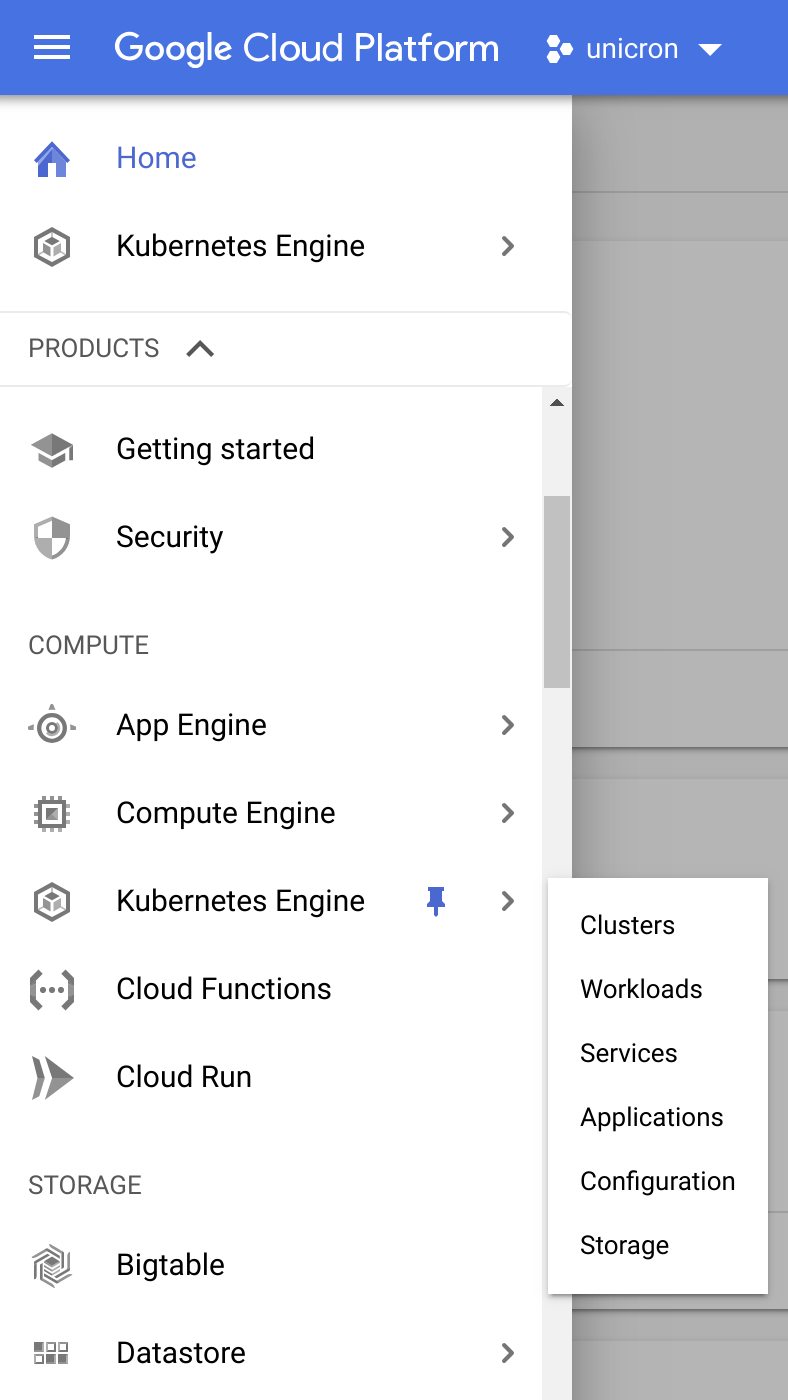
\includegraphics[width=0.5\textwidth]{figures/gke-setup-1.png}
    \caption{Select Kubernetes Engine then select Clusters}
    \label{fig:https-handshake}
\end{figure}

\FloatBarrier

This will bring you into the Kubernetes engine screen where you can then create your own cluster from scratch.

\begin{figure}[!h]
  \centering
    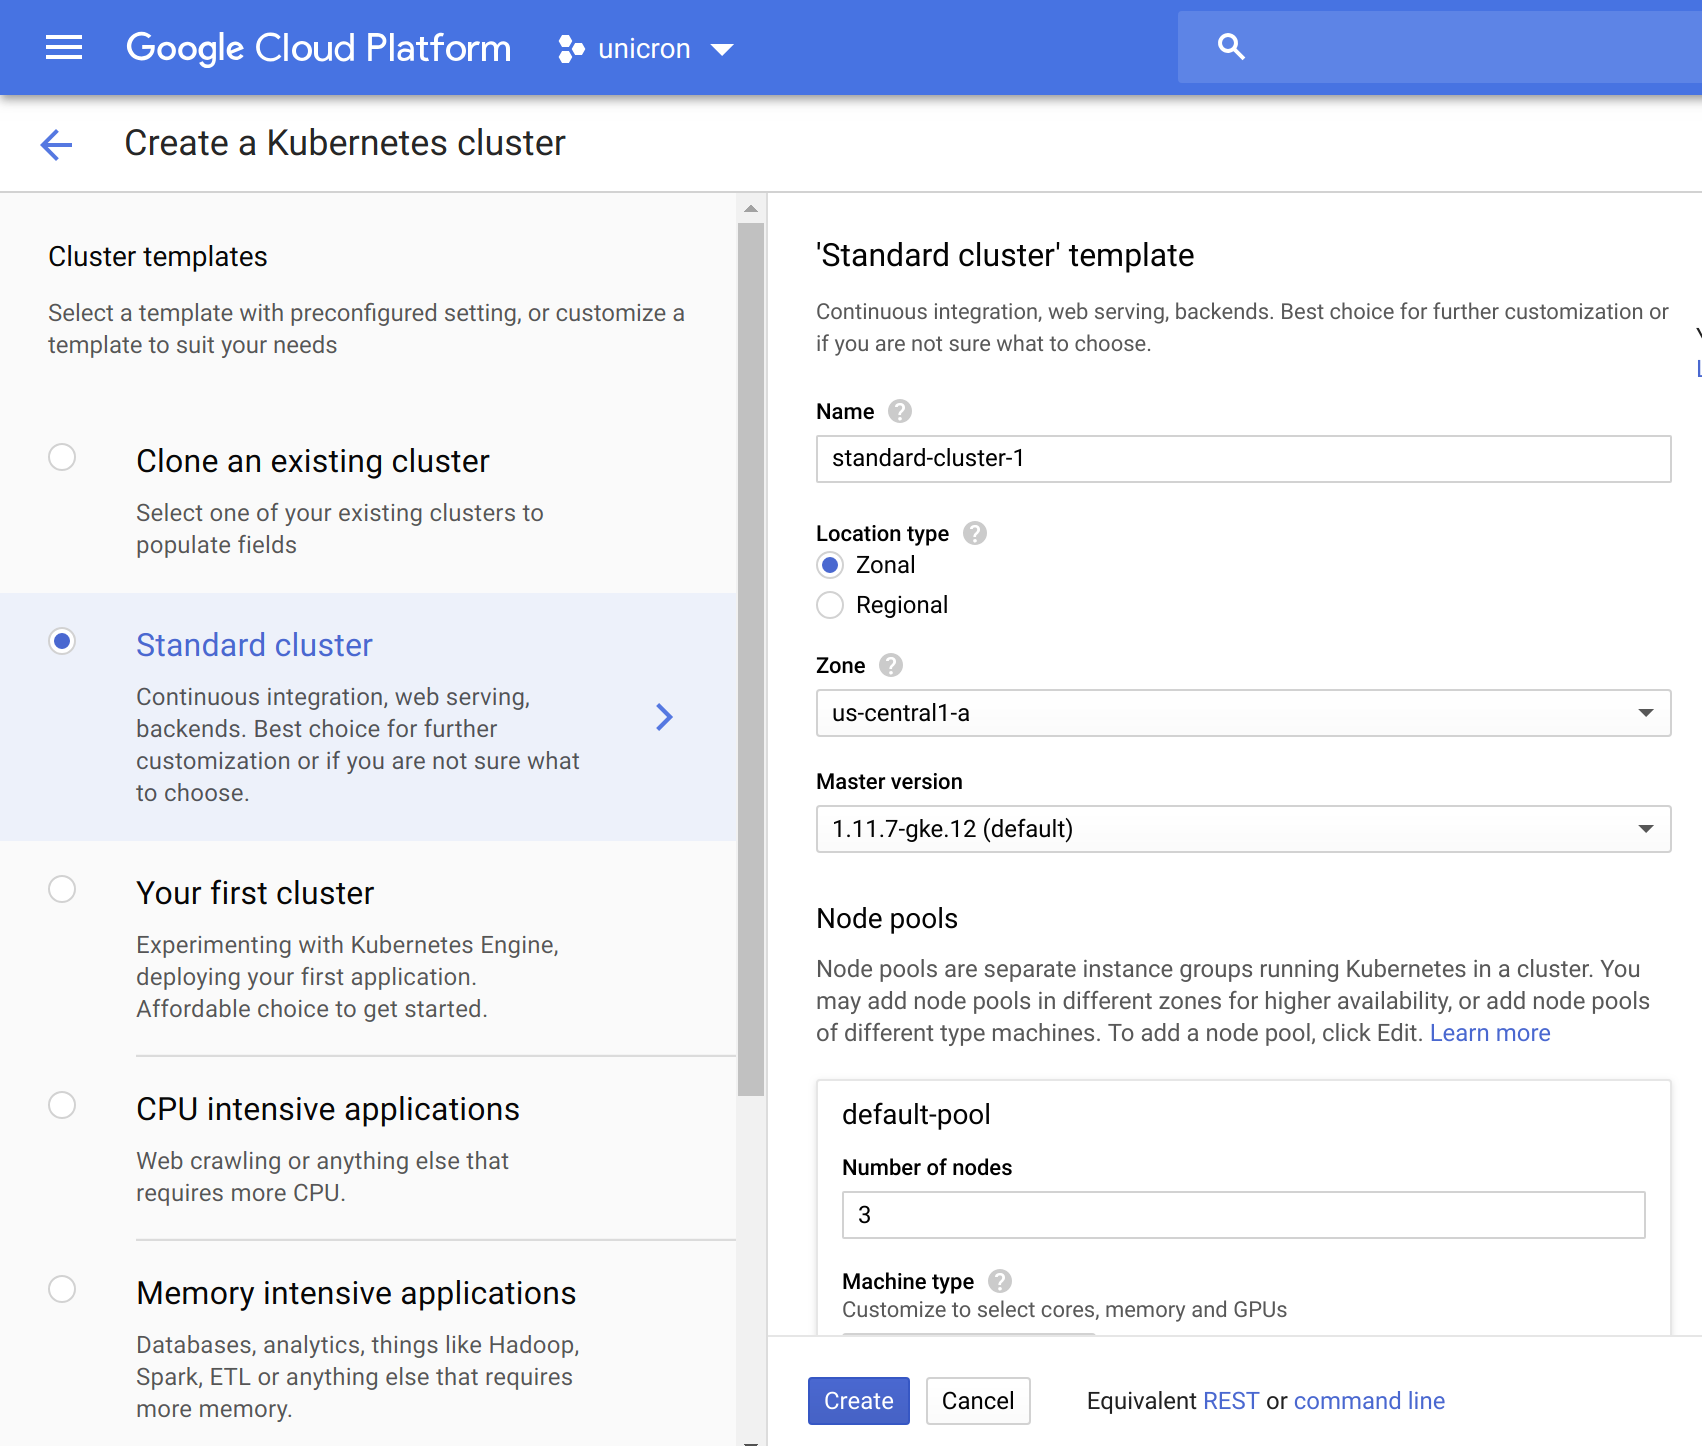
\includegraphics[width=0.8\textwidth]{figures/gke-setup-2.png}
    \caption{Select the resources to assign to this cluster}
    \label{fig:https-handshake}
\end{figure}

\FloatBarrier

Once you have selected your desired cluster resources, click Create and in a few minutes, your cluster should be created. Once the cluster is the setup you will be given the opportunity to connect to it. 

\begin{figure}[!h]
  \centering
    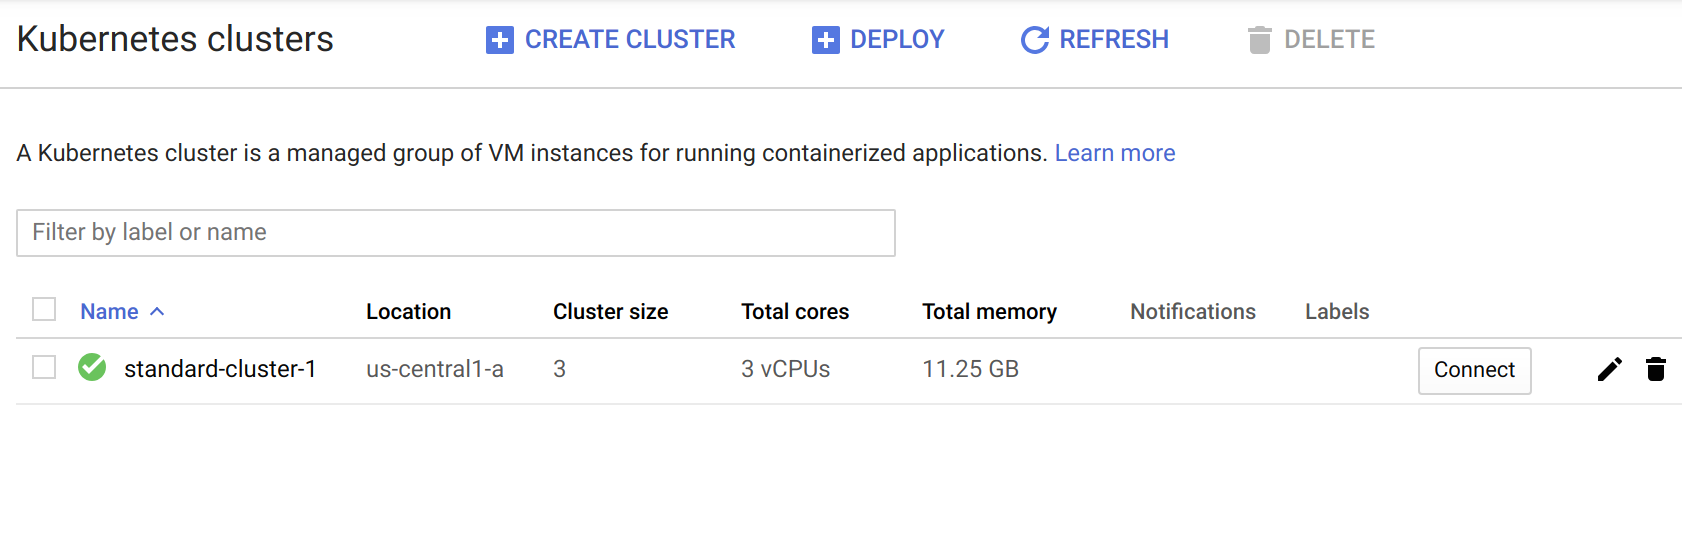
\includegraphics[width=0.8\textwidth]{figures/gke-setup-3.png}
    \caption{Click the connect button to get instructions on how to connect}
    \label{fig:https-handshake}
\end{figure}

\FloatBarrier

After clicking connect you will be given a command that you can run on your machine. Before running this command you will need to install the Google Cloud SDK tools. There is a quickstart guide available
\href{https://cloud.google.com/sdk/docs/quickstart-linux}{here}. Once you have installed the SDK tools then use the command that you have been given from the GKE console and you should be able to connect.

\subsection{Providing a scripting interface}

To ensure that it is possible to test a web socket server in a number of scenarios, the ws-flare platform allows users to essentially script how they want the test to progress. This enables the user to simulate a lot more scenarios than just simulating a number of connections at a time. When users create a new task with the platform they will be offered the opportunity to add a script. The script itself is a JSON array. An example of a valid script is below.

\begin{minted}{JSON}
[
    {
        "start": 0,
        "timeout": 55,
        "totalSimulators": 10000,
        "target": "wss://ws-flare-test-server.cfapps.io:4443"
    },
    {
        "start": 60,
        "timeout": 30,
        "totalSimulators": 5000,
        "target": "wss://ws-flare-test-server.cfapps.io:4443"
    },
    {
        "start": 120,
        "timeout": 60,
        "totalSimulators": 15000,
        "target": "wss://ws-flare-test-server.cfapps.io:4443"
    }
]
\end{minted}

In this scenario, we will initially be simulating 10000 connection o a web socket server. After 55 seconds, those 10000 connections will disconnect and one minute into the test another 5000 connection will attempt to connect to the server and disconnect after 30 seconds. Finally, 2 minutes into the test 15000 connection will be simulated for one minute. Scripting is a very powerful feature of the stress testing platform. 

One scenario we hope to detect with scripting is the ability for a web socket server to actively clean up after itself when users disconnect. One scenario we found recently where this would have been applicable is having a web socket server backed by a Redis database. The role of the web socket server was to send notifications. Whenever a new web socket connected to the server the web socket server would create a new connection to the Redis database to wait for notifications. We noticed every hour the application would crash and restart automatically. After some investigation, it was found that the Redis connections were never dropped when a user disconnected their web socket. Over time the web socket server would simply be starved of memory and crash. With this scripting ability, we can actively test for this kind of scenario, among many other scenarios.

\subsection{Pivotal Cloud Foundry Monitoring}

As mentioned already, Cloud Foundry exposes a powerful API. As a ws-flare test is in progress the platform will actively attempt to gain valuable metrics from this API. The first thing that happens when the test begins is that the system will attempt to log into cloud foundry using the user provided email and password. The login API endpoint request code is below

\begin{minted}{typescript}
async login(authorization_endpoint: string): Promise<Token> {
    const token = await post('https://api.run.pivotal.io
/oauth/token', {
            headers: {
                Authorization: 'Basic Y2Y6',
                'Content-Type': 'application/x-www-form-urlencoded'
            },
            json: true,
            form: {
                grant_type: 'password',
                client_id: 'cf',
                username: this.cfUser,
                password: this.cfPass
            }
        });

    return token.content as any;
}
\end{minted}

Using this code we can get an access token that can be used to query the endpoints we need. A few important points, we need to set Basic Y2Y6 as an Authorization header and the correct Content-Type. It is also necessary to specify the grant\_type which in this case is password. Cloud Foundry offers a number of grant types such as password and Oauth. 

Cloud Foundry is split up into 3 logical entities. These are

\begin{itemize}
  \item Organizations
  \item Spaces
  \item Applications
\end{itemize}

Organizations represent a department in a company. The organization is the entity that is billed for the resources used on Cloud Foundry. On PWS (Pivotal Web Services) which is Pivotal's cloud offering of Cloud Foundry this is measured in both CPU usage and Memory usage over a period of a month.

Spaces represent different environments. Spaces make environment repeat-ability very simple. For example you could have a DEV, STAGING and PROD environment all with the same applications deployed and utilizing the same resources, however, they are used for very different things. The DEV environment can be used by developers for testing code changes. The STAGING environment can be used by a quality assurance team to test any new features before reaching the PROD environment. the PROD environment is the last stop and this is the environment that the end user will be connecting to.

Just like there can be multiple spaces in an organization, there can also be multiple applications deployed in space. The applications themselves are the applications that a developer write. Applications on Cloud Foundry run in droplets, which are akin to Docker containers. Droplets require a user to specify a buildpack. Buildpacks are runtime environments for an application. Cloud Foundry supports many buildpacks for many different languages such as Java and NodeJS. To deploy an application to cloud foundry a user only needs to have an account and a manifest.yml file in the root of their project. A typical manifest file for a JAVA project might look like.

\begin{minted}{YAML}
name: cardsec
instances: 1
memory: 1024M
path: build/libs/cardsec-0.0.1-SNAPSHOT.jar
buildpack: java_buildpack
\end{minted}

The name represents the name of the application on cloud foundry. The instances are the number of running instances of the application, this allows users to easily scale up their applications under heavy load. The memory field is the total amount of memory that this app is allowed to consume. If this limit is exceeded then an application will likely crash with an out of memory exception. The path is the path to the generated jar file for this Java project and the buildpack is the desired run time environment, which in this case is Java.

Once ws-flare has gained access to cloud foundry we can now use the token to interrogate applications running within a specified space. Each running application has a unique GUID assigned to it. To find these unique ids we first need to find which organization and space the applications are running in. We first retrieve the list of organizations using the code below

\begin{minted}{typescript}
var response = json('https://api.run.pivotal.io/v2/organizations', {
    headers: {
        Authorization: token.token_type + ' ' + token.access_token,
        Accept: "application/json"
    }
});
\end{minted}

This will yield a list of organizations running in Cloud Foundry that the user has access to. Each organization also has a unique GUID. Once we find the correct GUID we can then use this to search for the correct space by using the code below.

\begin{minted}[breaklines]{typescript}
var response = json('https://api.run.pivotal.io/v2/organizations/' + orgId + '/spaces', {
    headers: {
        Authorization: token.token_type + ' ' + token.access_token,
        Accept: "application/json"
    }
});
\end{minted}

This will yield a list of spaces. Again each space has a unique GUID which we can use to get all the applications running within a space. To get a list of applications running within a space we can use the following code

\begin{minted}[breaklines]{typescript}
var response =  json('https://api.run.pivotal.io/v2/spaces/' + spaceId +'/apps', {
    headers: {
        Authorization: token.token_type + ' ' + token.access_token
    }
});
\end{minted}

Once the correct apps are found the last step is to use the obtained app GUID to get application statistics such as CPU and Memory usage. It is also possible to query the state of the application. There are 3 application states possible, these are, RUNNING, STOPPED and CRASHED. To get the information about a running application the code below is used. 

\begin{minted}[breaklines]{typescript}
json('https://api.run.pivotal.io/v2/apps/' + appId + '/stats', {
    headers: {
        Authorization: token.token_type + ' ' token.access_token
    }
});
\end{minted}

An example of a response from this endpoint is detailed below

\begin{minted}[breaklines]{JSON}
{
  "0": {
    "state": "RUNNING",
    "isolation_segment": "iso-seg-name",
    "stats": {
      "usage": {
        "disk": 66392064,
        "mem": 29880320,
        "cpu": 0.13511219703079957,
        "time": "2014-06-19 22:37:58 +0000"
      },
      "name": "app_name",
      "uris": [
        "app_name.example.com"
      ],
      "host": "10.0.0.1",
      "port": 61035,
      "uptime": 65007,
      "mem_quota": 536870912,
      "disk_quota": 1073741824,
      "fds_quota": 16384
    }
  }
}
\end{minted}

As can be seen in the response, there are some very useful metrics here. The cloud foundry monitor client will continue to poll this endpoint for the duration of the stress test. Polling will take place every second. All results from a successful request are stored in a MySQL database for displaying the results over a period of time.

\section{Stress testing the web socket server}

For connecting to a live web socket server we have chosen to utilize a popular NodeJS client called \href{https://www.npmjs.com/package/ws}{ws}. This is an intuitive client that has many useful features and hooks. For the purposes of this project, we will be monitoring certain metrics of a live web socket server. We will be monitoring the following metrics.

\begin{itemize}
  \item Successful connection over a period of time
  \item Failed connections
  \item Dropped connections
\end{itemize}

NodeJS ws client offers a few useful hooks when it comes to checking if a connection has successfully connected, failed or dropped. 

\begin{minted}[breaklines]{typescript}
const ws = new WebSocket('ws://www.host.com/path');
 
ws.on('open',  () => console.log('Successfully connected'));

ws.on('error',  () => console.log('Connection failed'));

ws.on('close' => console.log('Connection dropped'));
\end{minted}

\subsection{Testing tools used}

Test Driven Development was used extensively throughout this project. The following tools were used for testing the various applications in the ws-flare system.

\begin{itemize}
  \item Yarn package manager for NodeJS 
  \item Mocha testing framework for NodeJS
  \item Docker for simulating MySQL and RabbitMQ
  \item CypressJS for end to end testing the user interface
  \item Jest for unit testing the user interface
  \item nyc for measuring typescript code coverage
\end{itemize}

For packaging each service into a docker container we made use of \href{https://travis-ci.org/}{travis-ci} as a continuous integration pipeline. This tool is popular in the open source community and integrates well with GitHub which is the source code repository used for this project. When changes are made to any of the services Travis-ci will automatically detect the changes and begin a build. Travis will detect if you have a .travis-ci.yaml configuration file on the root of your project. An example of a Travis configuration file is outlined below.

\begin{minted}[breaklines]{yaml}
language: node_js
node_js:
  - '8'
services:
  - docker
install:
  - yarn --ignore-engines
  - docker pull mysql:5
script:
  - yarn test
  - docker build -t wsflare/ws-flare-projects-api:\$TRAVIS_BUILD_NUMBER .

after_success: yarn coverage

deploy:
  - provider: script
    script: docker login -u "\$DOCKER_USERNAME" -p "\$DOCKER_PASSWORD" && docker push wsflare/ws-flare-projects-api
    on:
      branch: master
\end{minted}

The build goes through a number of steps. First, it will install all dependencies of the service using Yarn package manager. Next, it will run all tests, failing the build if any test fails. Next, it will run a docker build which attempts to put our application into a docker container. Once this completes successfully Travis will release the docker container to docker hub which is a public registry for Docker containers. From there the docker container can be pulled into any project which is using docker or Kubernetes.

For monitoring code coverage this project uses a cloud offering called \href{https://coveralls.io/}{coveralls}. This integrates with Travis-ci. Code overage metrics are gathered during builds and sent to coveralls for analysis. Coveralls then summarises the code coverage for the project gives an overall code coverage metric ranging from 0 to 100\%. Coveralls is free to use with open source projects. % Solution design and implementation

\chapter{Results and Observations}
\lhead{\emph{Results and Observations}}

In this section the we will present the results of the experiments that we have conducted. For each experiment we will outline how the the experiment was setup, what technologies we are testing and also give an unbiased overview of the data gathered.

\section{Stress Testing}

For the first experiment we will be conducting a number of stress tests on three separate programming language WebSocket implementations. The implementation of each WebSocket server will be the vanilla example given from each of the implementations GitHub pages. Each of the experiments in this section will be using the  kubernetes setup as shown in table \ref{table:kubernetes-setup-experminent-1}

\begin{table}[H]
\resizebox{\textwidth}{!}{%
\begin{tabular}{llll}
\rowcolor[HTML]{ECF4FF} 
Machine Type          & Nodes & Total VCpus & Total Memory \\
small (1 Shared VCpu) & 10    & 10          & 16.99GB     
\end{tabular}%
}
\caption{Kubernetes Setup}
\label{table:kubernetes-setup-experminent-1}
\end{table}

\subsection{NodeJS Websocket Server}

For NodeJS we will be using a popular library called WS. The code for the server is outlined in code section \ref{table:nodejs-server-experiment-1}

\begin{listing}[H]
    \caption{NodeJS Websocket Server Implemntation}
    \label{table:nodejs-server-experiment-1}
    \begin{minted}{Javascript}
const http = require('http');
const WebSocket = require('ws');

console.log('Starting ws server');

const server = http.createServer();
const wss = new WebSocket.Server({noServer: true});

wss.on('connection', (ws) => {
    console.log('new connection');

    ws.on('close', () => {
        console.log('connection dropped');
    });
});

server.on('upgrade', function upgrade(request, socket, head) {
    wss.handleUpgrade(request, socket, head, function done(ws) {
        wss.emit('connection', ws, request);
    });
});

server.listen(process.env.PORT || 3000);
\end{minted}
\end{listing}

The NodeJS server as listed in \ref{table:nodejs-server-experiment-1} code required to handle HTTP upgrades to websocket manually as Cloud Foundry does not automatically handle the HTTP upgrade.

The NodeJS WebSocket server is deployed on cloud foundry with the resource limits specified in table \ref{table:cf-resource-limits-1}

\begin{table}[H]
\resizebox{0.7\textwidth}{!}{%
\begin{tabular}{ll}
\rowcolor[HTML]{ECF4FF} 
Instances & Memory Limit Per Instance \\
1         & 64MB                     
\end{tabular}%
}
\caption{Cloud Foundry Resource Limits}
\label{table:cf-resource-limits-2}
\end{table}

The initial test will use the following ws-flare script to simulate 1000 users over a period of 60 seconds

\begin{listing}[H]
    \caption{WS-Flare test script for 1000 users}
    \label{table:nodejs-server-experiment-1}
    \begin{minted}{json}
[
    {
        "start": 0,
        "timeout": 60,
        "totalSimulators": 1000,
        "target": "wss://ws-flare-test-server.cfapps.io:4443"
    }
]
\end{minted}
\end{listing}

\begin{figure}[H]
  \centering
    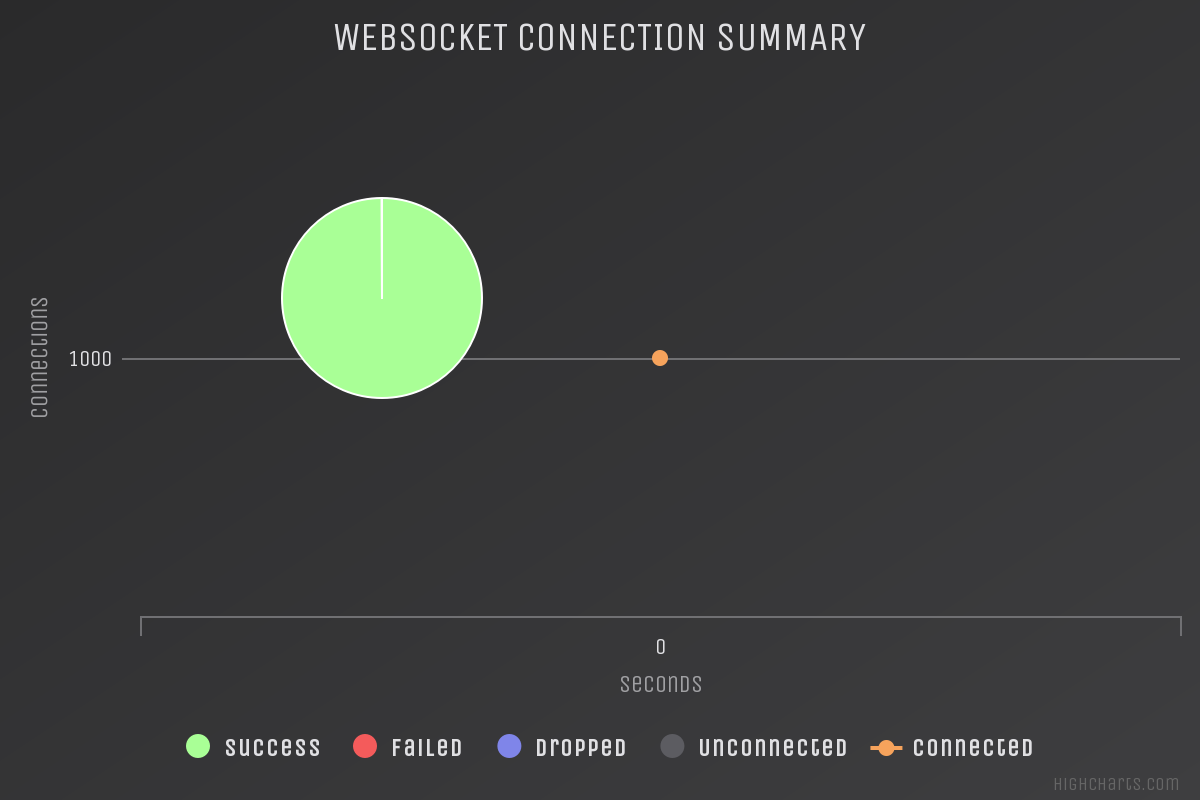
\includegraphics[width=0.8\textwidth]{figures/experiments/experiment-1/node-js/conn-summary-1000.png}
    \caption{Results of simulating 1000 websockets}
    \label{fig:experiment-1-conn-summary-1000}
\end{figure}

\begin{figure}[H]
  \centering
    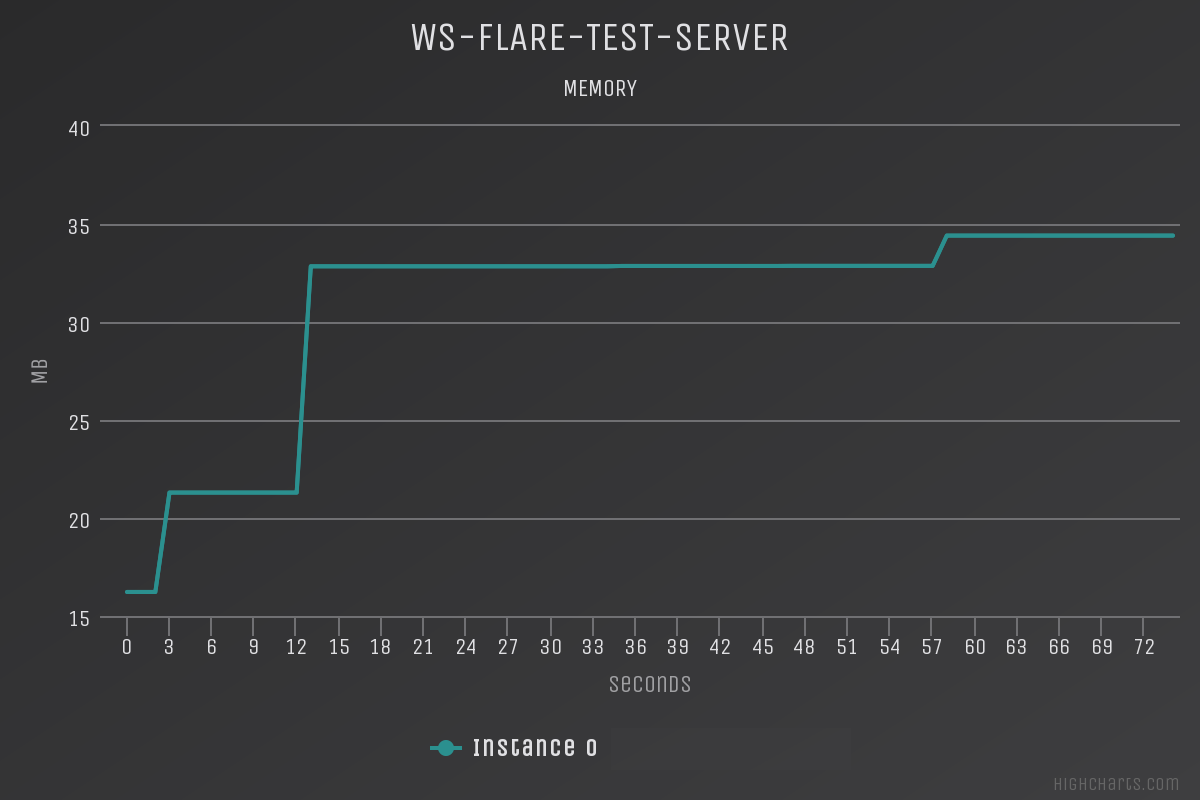
\includegraphics[width=0.8\textwidth]{figures/experiments/experiment-1/node-js/memory-1000.png}
    \caption{Memory consumption of websocket server testing 1000 connections}
    \label{fig:experiment-1-memory-1000}
\end{figure}

\begin{figure}[H]
  \centering
    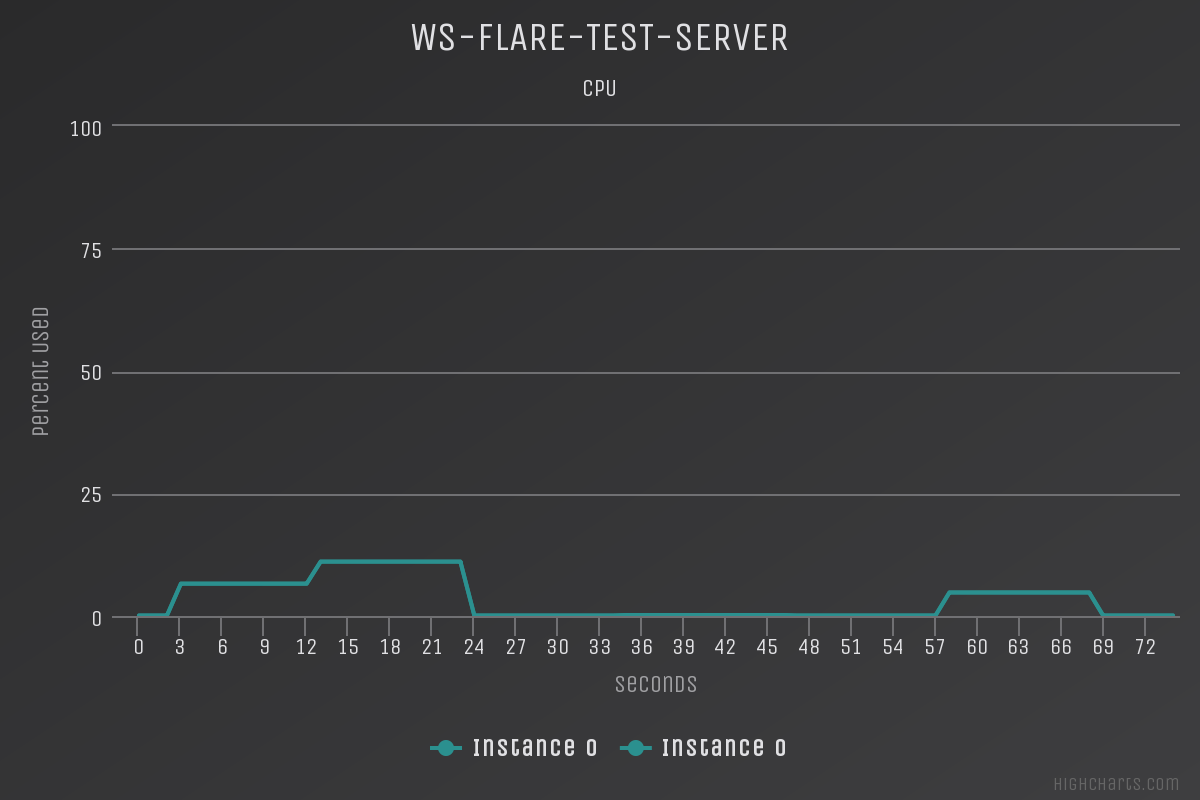
\includegraphics[width=0.8\textwidth]{figures/experiments/experiment-1/node-js/cpu-1000.png}
    \caption{CPU consumption of websocket server testing 1000 connections}
    \label{fig:experiment-1-cpu-1000}
\end{figure}

As can be seen from figure \ref{fig:experiment-1-conn-summary-1000} simulating 1000 users has a 100\% success rate.

In figure \ref{fig:experiment-1-memory-1000} and figure \ref{fig:experiment-1-cpu-1000} the memory and CPU resources are outlined as the test is in progress. We can see that the memory gradually rises from 16(MB) to 34 (MB). The CPU consumption remains stable throughout the test, reaching a maximum of 11\% usage. This occurred as the websockets were initializing the connection to the server, suggesting that the most resource intensive time occurs when making the initial connection. After all connections have been made we then see the CPU return to 0\% usage. 

\subsubsection{5000 Connections}

1000 users connecting at the same time is a good expectation for websites that are not expecting a lot of traffic. Lets increase this to 5000 users using the script in listing \ref{table:nodejs-server-experiment-2}

\begin{listing}[H]
    \caption{WS-Flare test script for 5000 users}
    \label{table:nodejs-server-experiment-2}
    \begin{minted}{json}
[
    {
        "start": 0,
        "timeout": 60,
        "totalSimulators": 5000,
        "target": "wss://ws-flare-test-server.cfapps.io:4443"
    }
]
\end{minted}
\end{listing}

\begin{figure}[H]
  \centering
    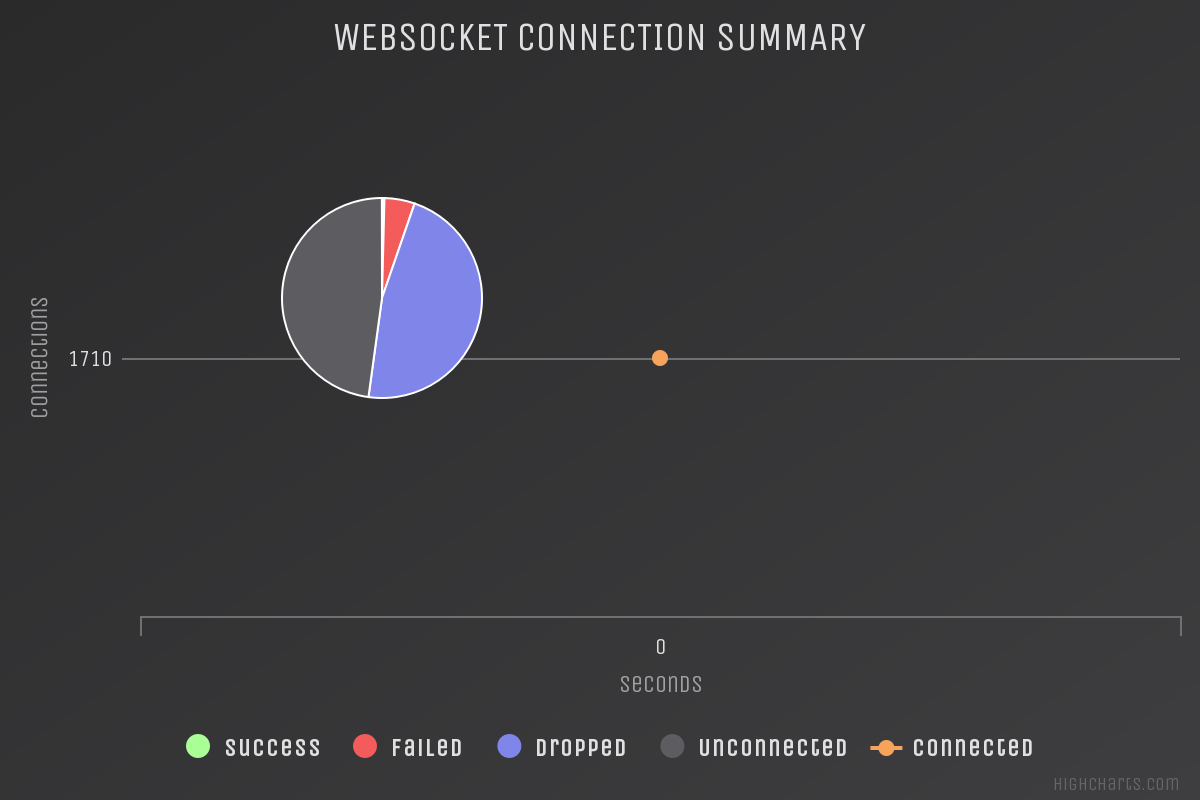
\includegraphics[width=0.8\textwidth]{figures/experiments/experiment-1/node-js/conn-summary-5000.png}
    \caption{Results of simulating 5000 websockets}
    \label{fig:experiment-1-conn-summary-5000}
\end{figure}

\begin{figure}[H]
  \centering
    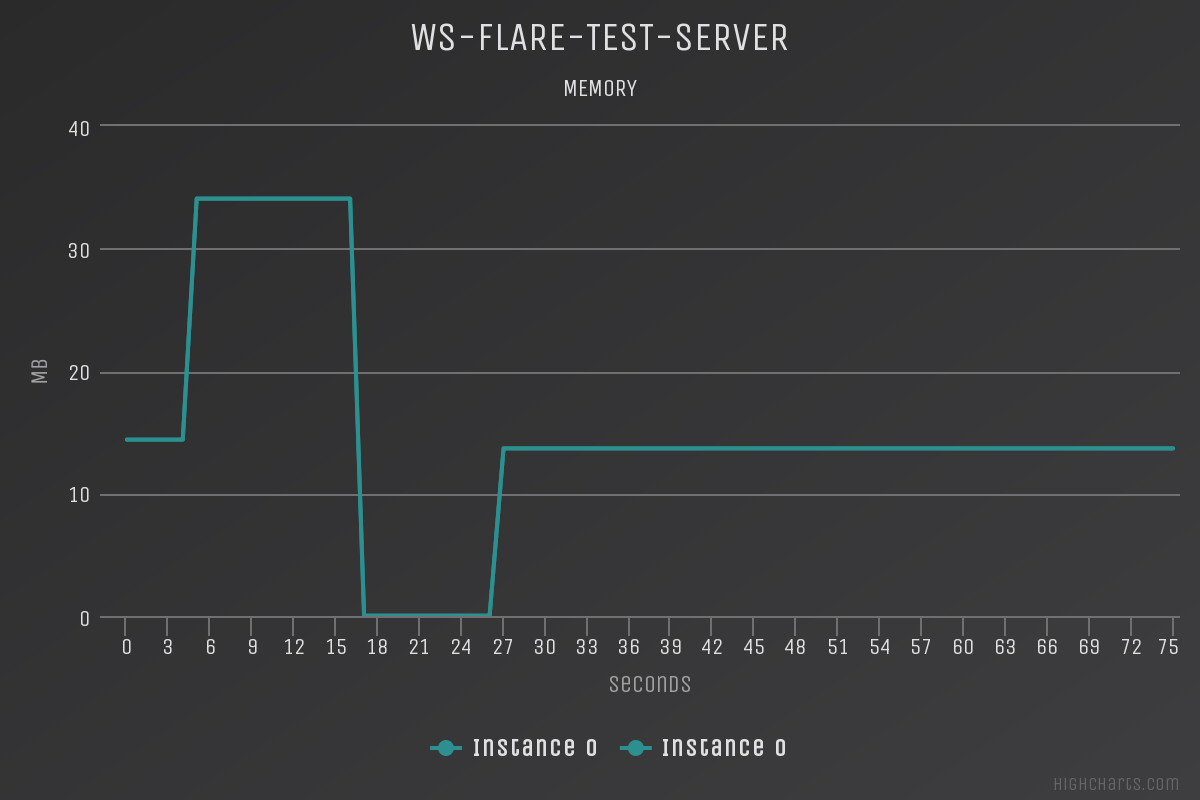
\includegraphics[width=0.8\textwidth]{figures/experiments/experiment-1/node-js/memory-5000.png}
    \caption{Memory consumption of websocket server testing 5000 connections}
    \label{fig:experiment-1-memory-5000}
\end{figure}

\begin{figure}[H]
  \centering
    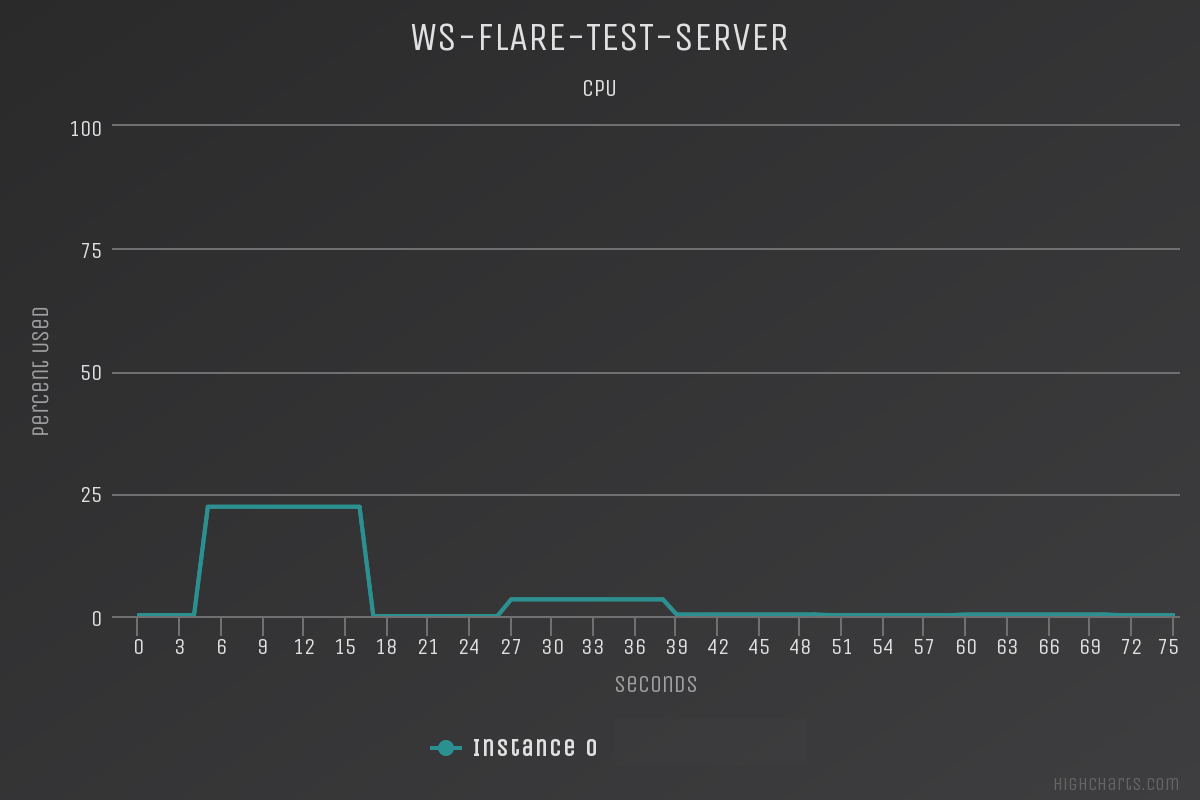
\includegraphics[width=0.8\textwidth]{figures/experiments/experiment-1/node-js/cpu-5000.png}
    \caption{CPU consumption of websocket server testing 5000 connections}
    \label{fig:experiment-1-cpu-5000}
\end{figure}

After increasing the test to simulate 5000 connections we see from figure \ref{fig:experiment-1-conn-summary-5000} that initially the test reached 1710 connections. After this was reached we see a big dip in memory in figure \ref{fig:experiment-1-memory-5000} and CPU in figure \ref{fig:experiment-1-cpu-5000}. The indicates that a 64(MB) limit of memory is not enough to handle this amount of WebSocket connections. One possible solution to this is to add more instances. Through trial and error we found that to reach 5000 users successfully connecting at the same time, one of the following resources are needed on Cloud Foundry

\begin{table}[H]
\resizebox{0.7\textwidth}{!}{%
\begin{tabular}{ll}
\rowcolor[HTML]{ECF4FF} 
Instances & Memory Limit Per Instance \\
4         & 64MB     \\
1         & 256MB     
\end{tabular}%
}
\caption{Cloud Foundry Resource Limits}
\label{table:cf-resource-limits-3}
\end{table}

\begin{figure}[H]
  \centering
    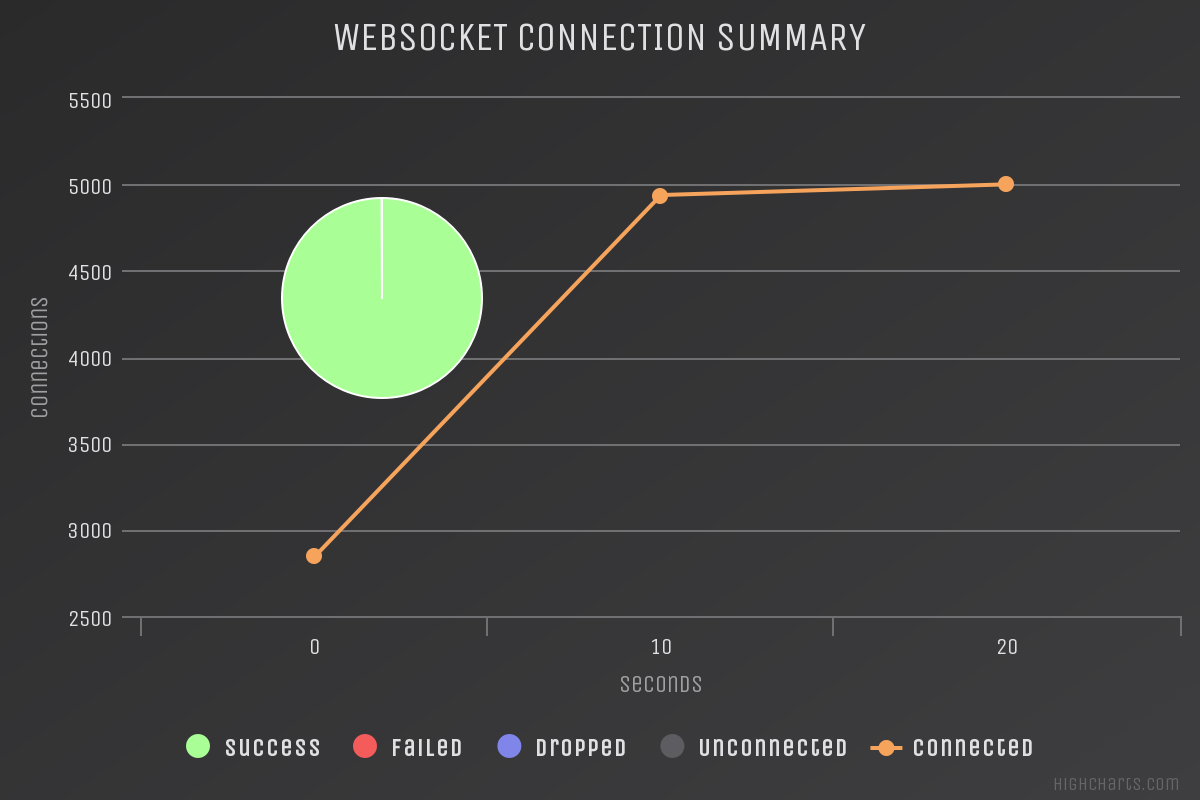
\includegraphics[width=0.8\textwidth]{figures/experiments/experiment-1/node-js/conn-summary-5000-4-instances.png}
    \caption{Results of simulating 5000 websockets with 4 instances}
    \label{fig:experiment-1-conn-summary-5000-4-instances}
\end{figure}

\begin{figure}[H]
  \centering
    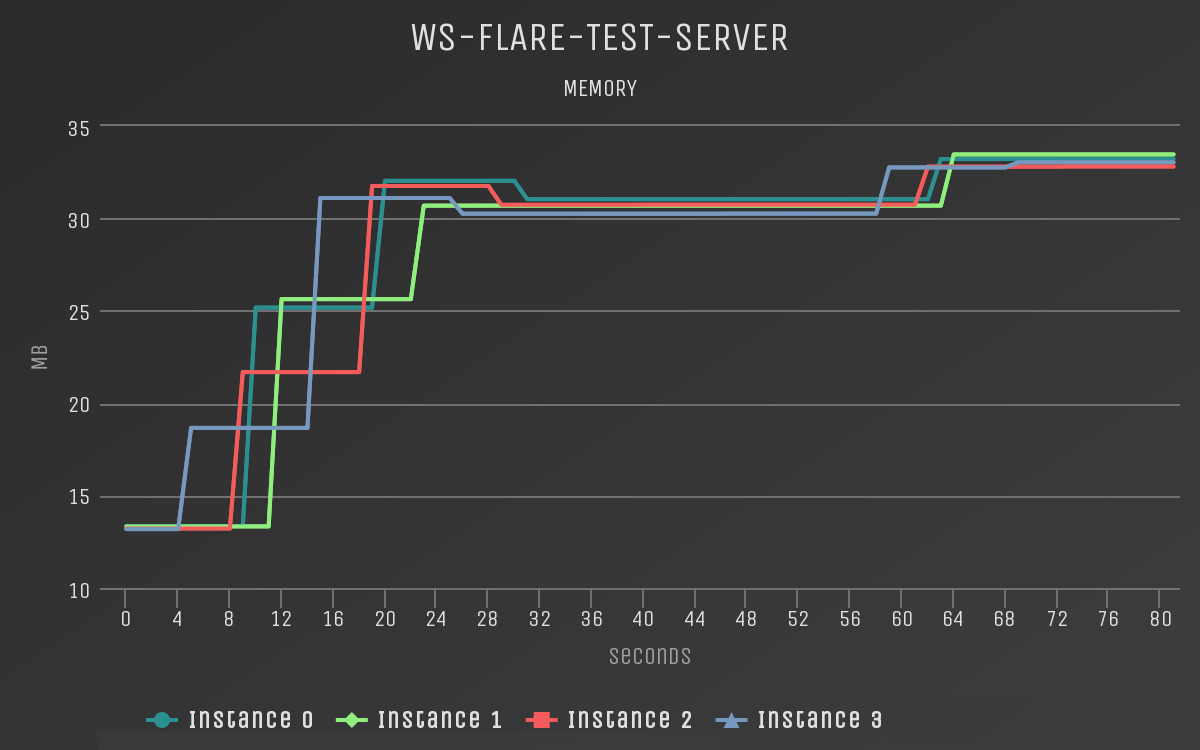
\includegraphics[width=0.8\textwidth]{figures/experiments/experiment-1/node-js/memory-5000-4-instances.png}
    \caption{Memory consumption of websocket server testing 5000 connections with 4 instances}
    \label{fig:experiment-1-memory-5000-4-instances}
\end{figure}

\begin{figure}[H]
  \centering
    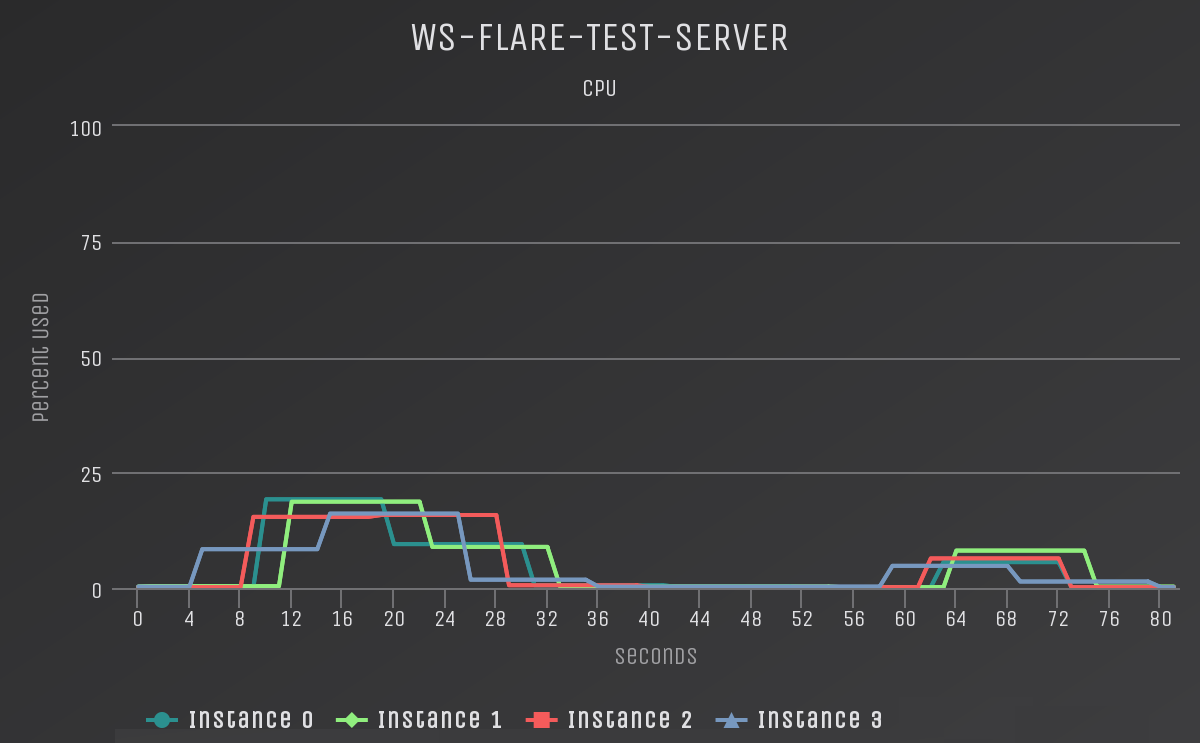
\includegraphics[width=0.8\textwidth]{figures/experiments/experiment-1/node-js/cpu-5000-4-instances.png}
    \caption{CPU consumption of websocket server testing 5000 connections with 4 instances}
    \label{fig:experiment-1-cpu-5000-4-instances}
\end{figure}

\begin{figure}[H]
  \centering
    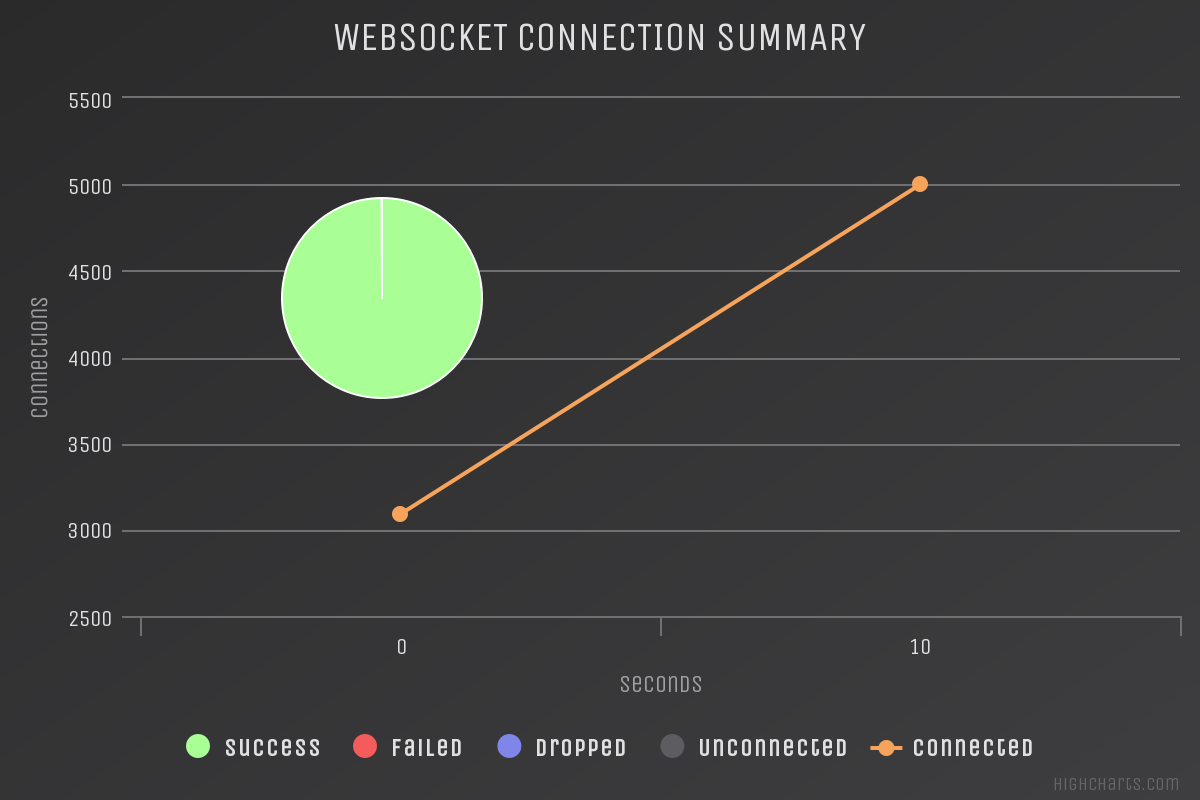
\includegraphics[width=0.8\textwidth]{figures/experiments/experiment-1/node-js/conn-summary-5000-256-memory.png}
    \caption{Results of simulating 5000 websockets with 256 MB of memory}
    \label{fig:experiment-1-conn-summary-5000-1-instances-256-mem}
\end{figure}

\begin{figure}[H]
  \centering
    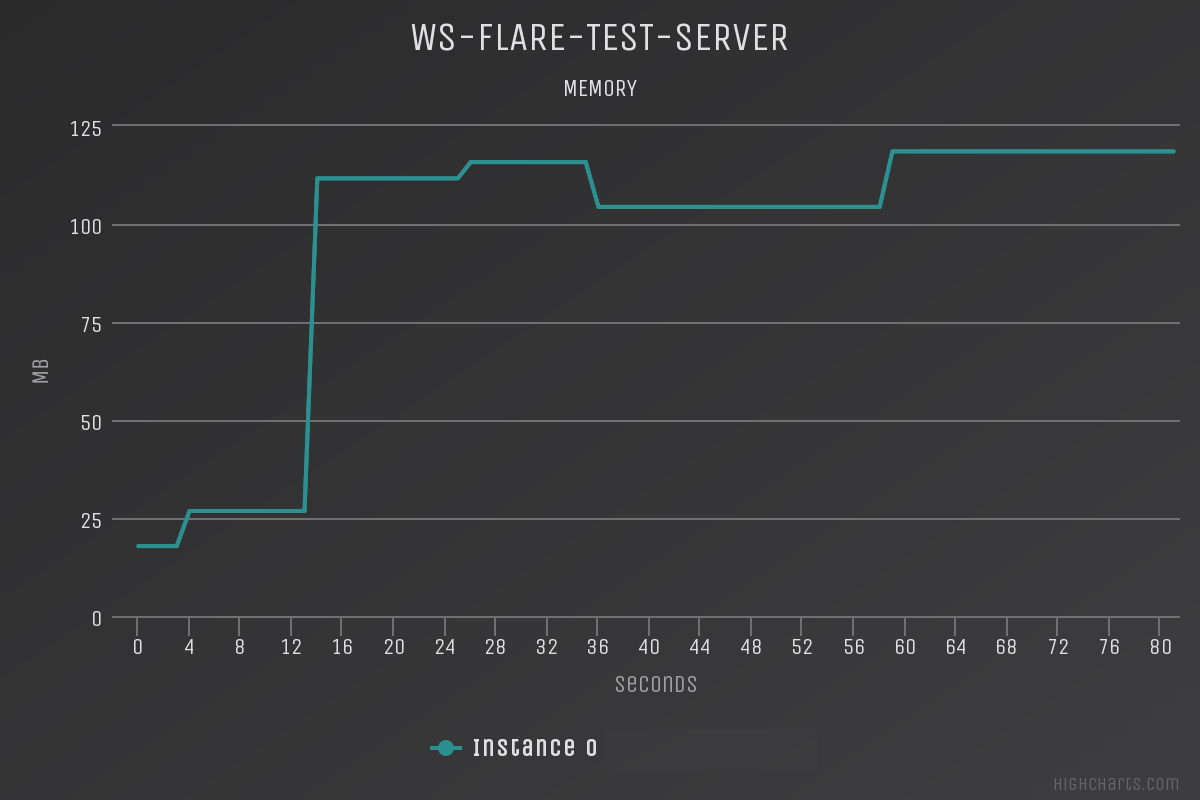
\includegraphics[width=0.8\textwidth]{figures/experiments/experiment-1/node-js/memory-5000-256-memory.png}
    \caption{Memory consumption of websocket server testing 5000 connections with 256 MB of memory}
    \label{fig:experiment-1-memory-5000-1-instances-256-mem}
\end{figure}

\begin{figure}[H]
  \centering
    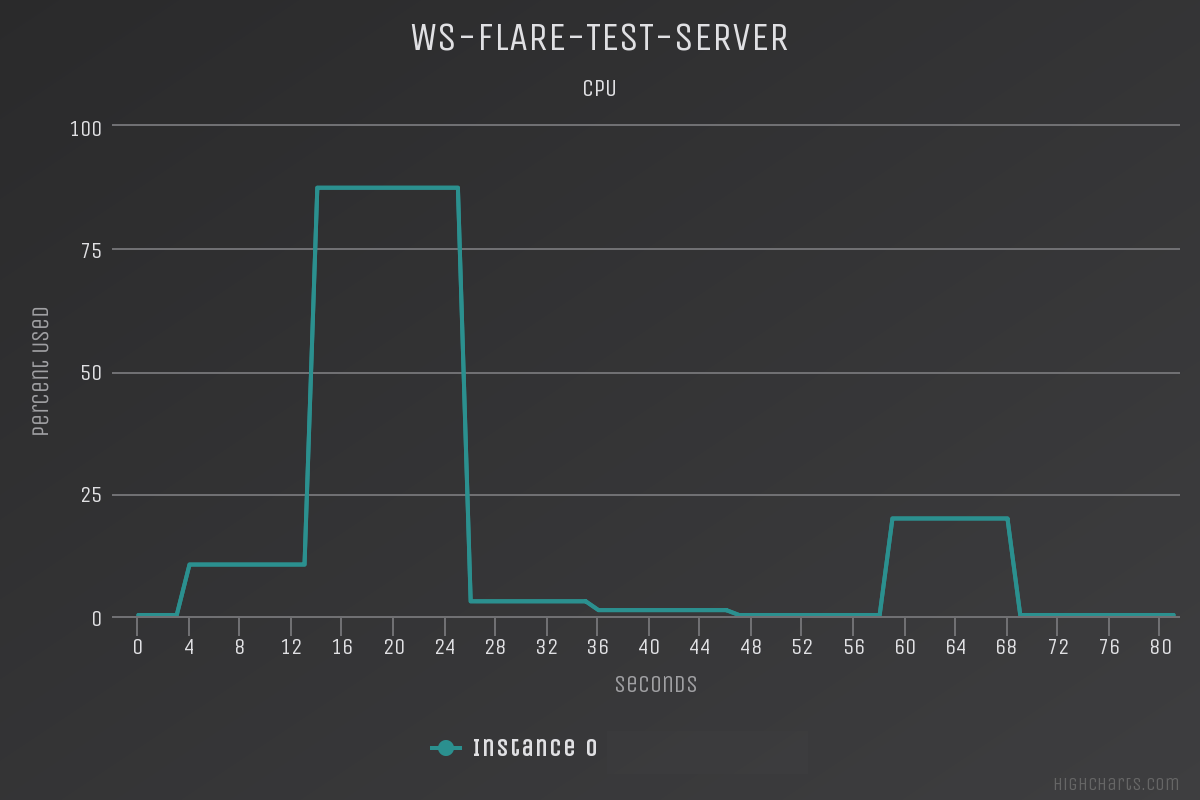
\includegraphics[width=0.8\textwidth]{figures/experiments/experiment-1/node-js/cpu-5000-256-memory.png}
    \caption{CPU consumption of websocket server testing 5000 connections with 256 MB of memory}
    \label{fig:experiment-1-cpu-5000-1-instances-256-mem}
\end{figure}

Comparing the CPU between using 4 instances of 64 MB of memory each in figure \ref{fig:experiment-1-cpu-5000-4-instances} with 1 instance and 256 MB of memory in figure \ref{fig:experiment-1-cpu-5000-1-instances-256-mem} we see that the with 1 instance 87\% memory consumption when connections were being estanblished. However with 4 instances the cpu usage reached a maximum of 19\% per instance. This is due to the load balancing in effect here. Due to this we recommend using 4 instances instead of 1. 

\subsubsection{30000 Connections}

For the next experiment we attempted 30000 users connecting at the same time. Using the script in \ref{listing:nodejs-server-experiment-3}

\begin{listing}[H]
    \caption{WS-Flare test script for 5000 users}
    \label{listing:nodejs-server-experiment-3}
    \begin{minted}{json}
[
    {
        "start": 0,
        "timeout": 60,
        "totalSimulators": 30000,
        "target": "wss://ws-flare-test-server.cfapps.io:4443"
    }
]
\end{minted}
\end{listing}

There will be 1 instance which is assigned a maximum of 2GB of memory as outlined in table \ref{table:cf-resource-limits-4}

\begin{table}[H]
\resizebox{0.7\textwidth}{!}{%
\begin{tabular}{ll}
\rowcolor[HTML]{ECF4FF} 
Instances & Memory Limit Per Instance \\
1         & 2GB     \\ 
\end{tabular}%
}
\caption{Cloud Foundry Resource Limits}
\label{table:cf-resource-limits-4}
\end{table}

\begin{figure}[H]
  \centering
    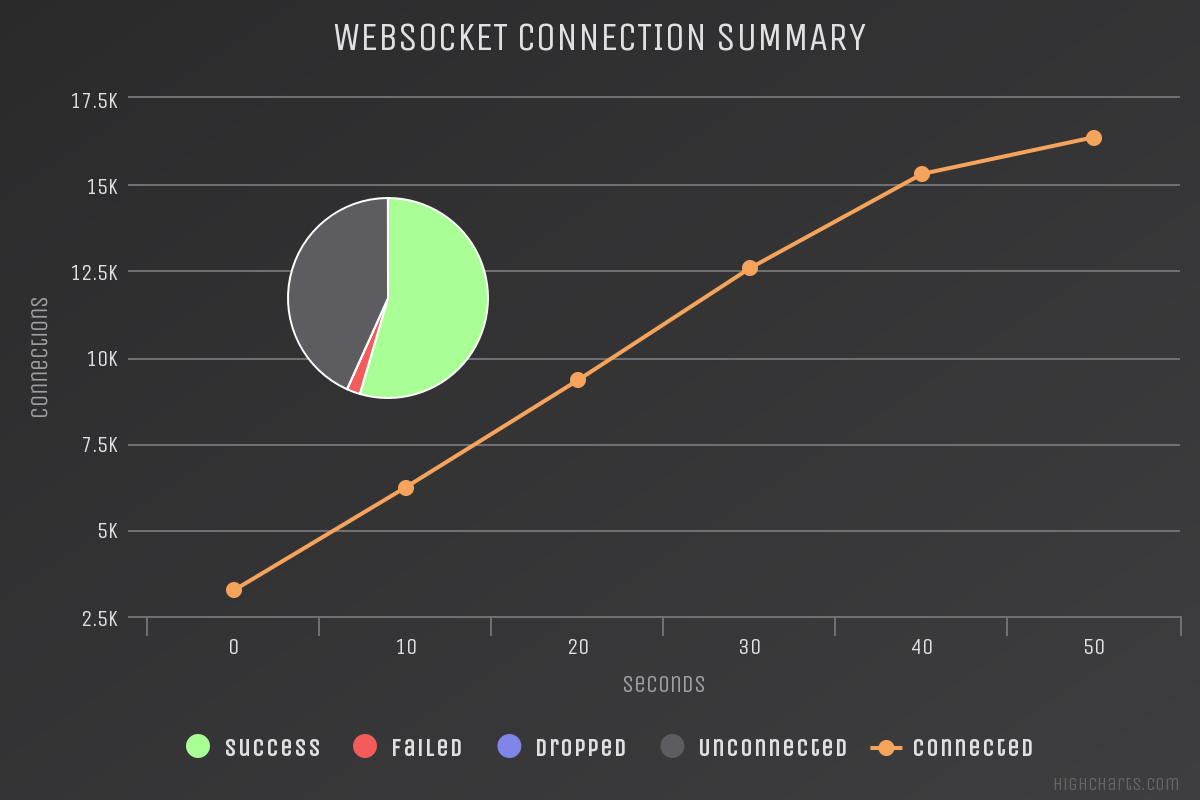
\includegraphics[width=0.8\textwidth]{figures/experiments/experiment-1/node-js/conn-summary-30000-256-memory.png}
    \caption{Results of simulating 30000 websockets with 256 MB of memory}
    \label{fig:experiment-3-conn-summary-5000-1-instances-256-mem}
\end{figure}

\begin{figure}[H]
  \centering
    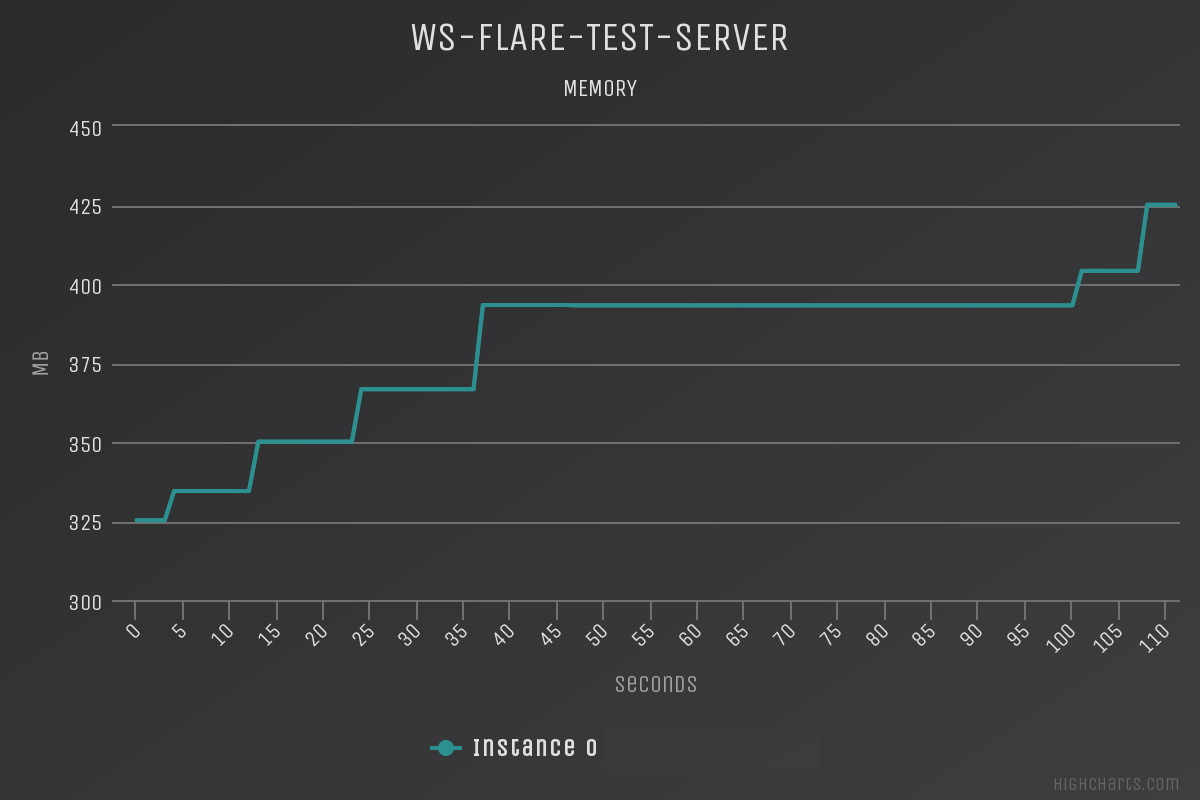
\includegraphics[width=0.8\textwidth]{figures/experiments/experiment-1/node-js/memory-30000-256-memory.png}
    \caption{Memory consumption of websocket server testing 30000 connections with 256 MB of memory}
    \label{fig:experiment-3-memory-5000-1-instances-256-mem}
\end{figure}

\begin{figure}[H]
  \centering
    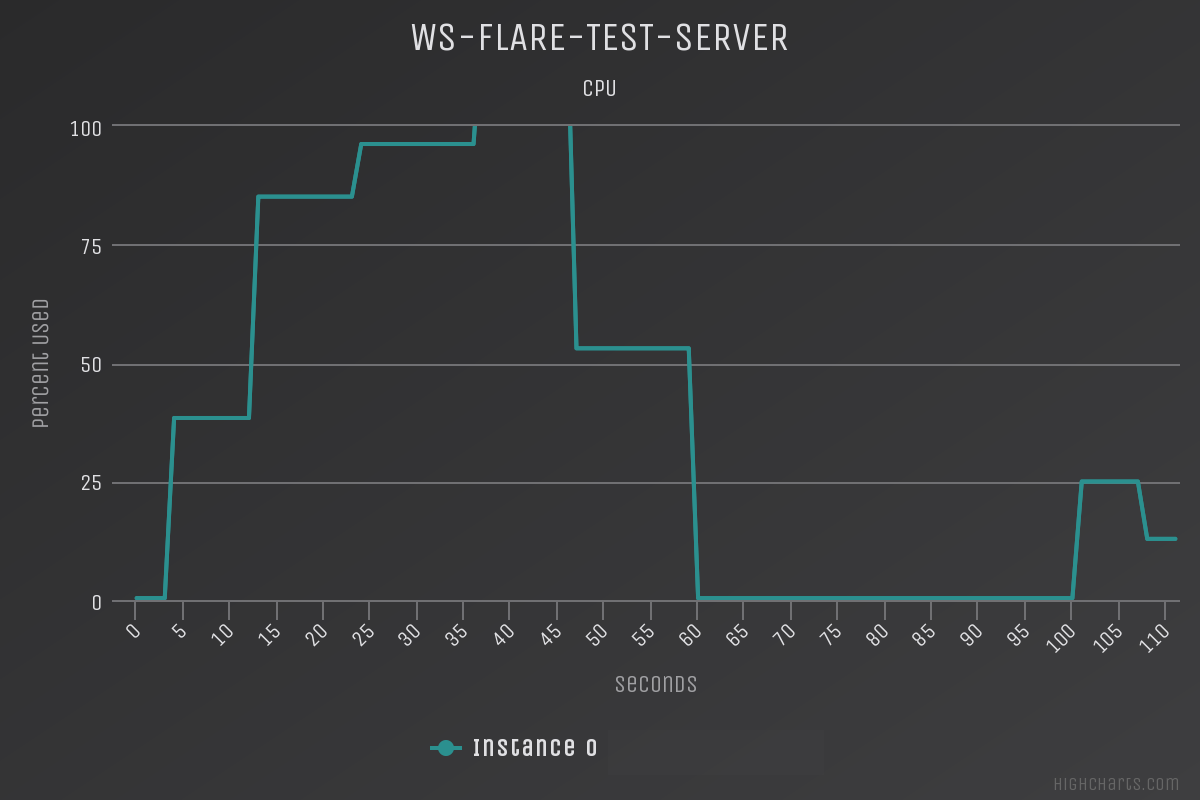
\includegraphics[width=0.8\textwidth]{figures/experiments/experiment-1/node-js/cpu-30000-256-memory.png}
    \caption{CPU consumption of websocket server testing 30000 connections with 256 MB of memory}
    \label{fig:experiment-3-cpu-5000-1-instances-256-mem}
\end{figure}

In figure \ref{fig:experiment-3-conn-summary-5000-1-instances-256-mem} we see that we did not reach the target of 30000 connections within the 60 second limit. Instead we reached 16365 connections. The reason for this becomes clear when we look at figure  \ref{fig:experiment-3-cpu-5000-1-instances-256-mem}. On 35 seconds in the CPU was at 120\% which goes over the 100\% limit imposed by Cloud Foundry. It is clear that this a single server is not enough to allow 30000 connections. We can keep adding more and more memory, however we are bound by the constraints of the CPU on Cloud Foundry, which means adding more memory would not achieve better results. Scaling to the resources defined in table \ref{table:cf-resource-limits-5} produced better results as can be seen in figure \ref{fig:experiment-3-conn-summary-30000-5-instances-512-mem}. There were 27764 successful connections and 2236 dropped connections.

\begin{table}[H]
\resizebox{0.7\textwidth}{!}{%
\begin{tabular}{ll}
\rowcolor[HTML]{ECF4FF} 
Instances & Memory Limit Per Instance \\
5         & 512MB     \\ 
\end{tabular}%
}
\caption{Cloud Foundry Resource Limits}
\label{table:cf-resource-limits-5}
\end{table}

\begin{figure}[H]
  \centering
    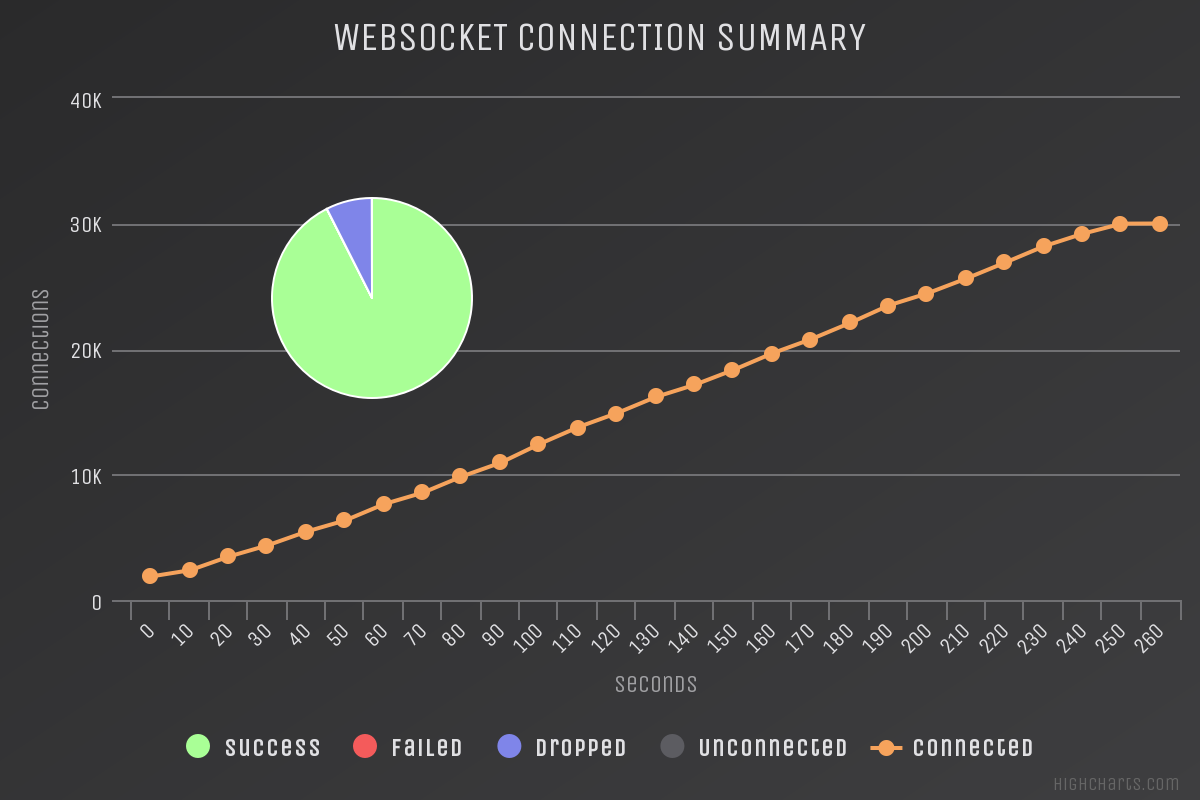
\includegraphics[width=0.8\textwidth]{figures/experiments/experiment-1/node-js/conn-summary-30000-5-instances-512-memory.png}
    \caption{Results of simulating 30000 websockets with 5 instances and 512 MB of memory}
    \label{fig:experiment-3-conn-summary-30000-5-instances-512-mem}
\end{figure}

\begin{figure}[H]
  \centering
    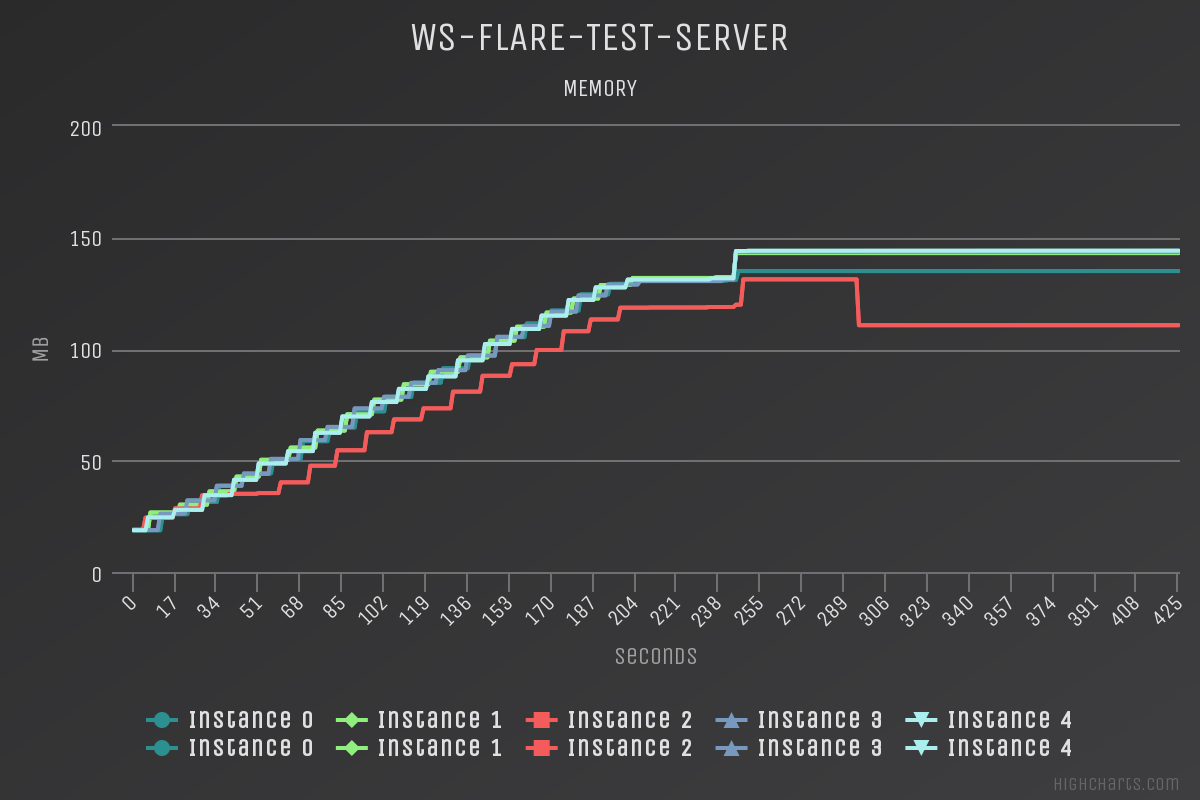
\includegraphics[width=0.8\textwidth]{figures/experiments/experiment-1/node-js/memory-30000-5-instances-512-memory.png}
    \caption{Memory consumption of websocket server testing 30000 connections with 5 instances and 512 MB of memory}
    \label{fig:experiment-3-memory-30000-5-instances-512-mem}
\end{figure}

\begin{figure}[H]
  \centering
    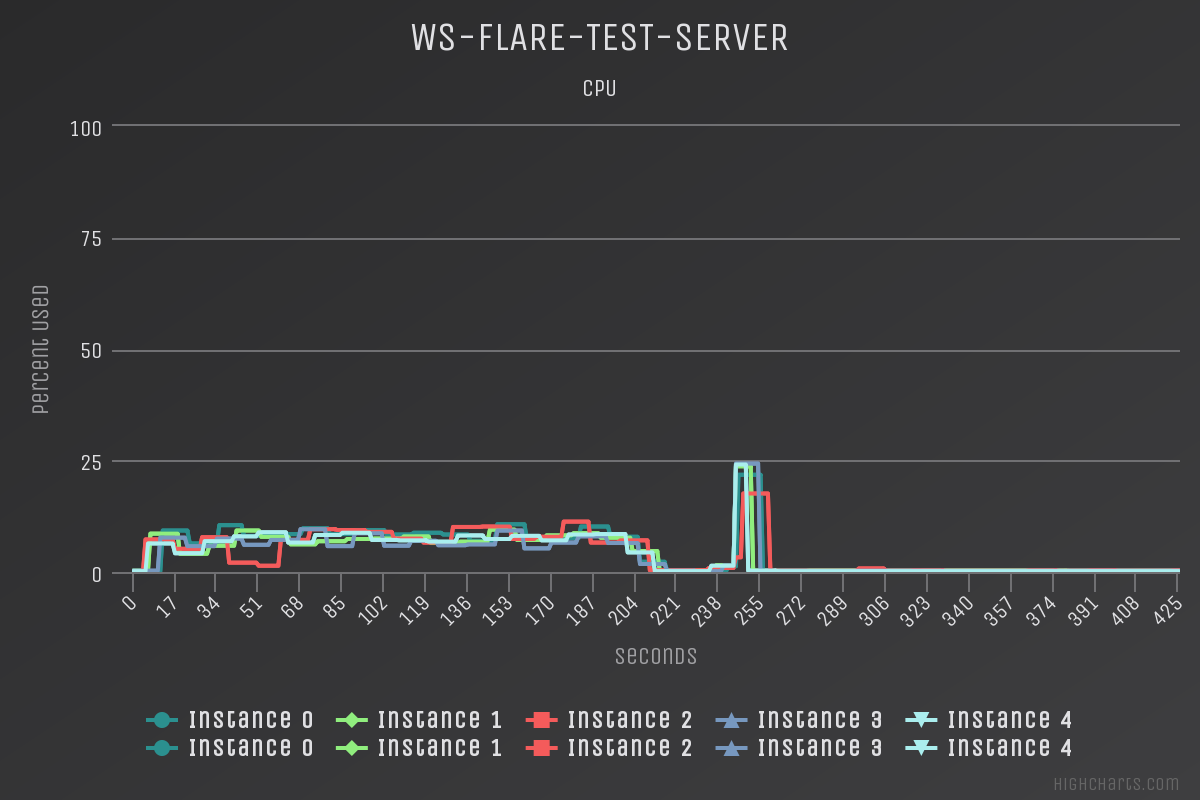
\includegraphics[width=0.8\textwidth]{figures/experiments/experiment-1/node-js/cpu-30000-5-instances-512-memory.png}
    \caption{CPU consumption of websocket server testing 30000 connections with 5 instances and 512 MB of memory}
    \label{fig:experiment-3-cpu-530000000-5-instances-512-mem}
\end{figure} % Results and Observations
%\chapter{Ethical Issues}
\lhead{\emph{Ethical Issues}}
If the proposed research directly involves human or live animal subjects, discuss the ethical issues involved and the actions that will be taken to ensure compliance with CIT ethics guidelines and with the CIT Child Protection Policy (if children are involved).

\chapter{Conclusions and Future Work}
\lhead{\emph{Conclusions and Future Work}}

\section{Discussion}

The purpose of this research project was to design and implement a WebSocket stress test tool that could easily be integrated into continuous integration environments as well as providing automated insights into the underlying microservices of a system under test.

In chapter 4 the results of our experimentation with the ws-flare platform were presented. The platform was tested against a variety of web socket and microservice implementations as well as testing compatibility with a number of third party continuous integration tools. 

The platform itself performed well in all experiments, however, it was surprising to see how little physical web socket connections NodeJS and GoLang could handle while deployed to Cloud Foundry. The maximum that could be achieved was just under 30000 connections. Even scaling those servers to many more instances had no real effect while attempting to go beyond this number. This raises the question, is Cloud Foundry imposing a limit on the number of connections that can be sent to servers deployed on their system. For most websites, 30000 connections is more than sufficient for their use cases, however for much larger sites such as Google and Facebook, PaaS systems such as Cloud Foundry or Heroku may not be able to handle the required traffic, which suggests that Cloud Foundry's target audience is small to medium scale businesses. Some reports suggest that NodeJS and can handle many hundreds of thousands of connections on a single server \cite{nodeConnections}. One such experiment even reached 600 thousand connections on a single Amazon Web Services server \cite{nodeConnections}. The difference here may be that connections to Cloud Foundry are shared between all subscribers to Pivotal Web Services. So it may not be possible to get the same throughput as would be seen in the case of a dedicated server like in the case of Amazon Web Services. 

Given more time on this project it would have been interesting to compare the connection limits between different systems such as Amazon Web Services, Google Kubernetes Engine, and Cloud Foundry. 

\section{Conclusion}

While it was surprising to see the low number of connections that could be achieved on Cloud Foundry, this dissertation has achieved its primary goal of creating a web socket stress test tool that can integrate into Cloud Foundry as well as continuous integration systems. 

This study also makes it clear that performance or stress testing environments are one of the most underutilized forms of testing, due to the complexities involved, especially when it comes to scaling to very large numbers of connections.

Another conclusion that can be drawn from this dissertation is that web sockets in microservices environments that communicate with multiple services can have a huge impact on CPU and Memory usage as well as affecting the overall stability of the entire system, even for simple examples, such as the experiment conducted in Chapter 4 with multiple services communicating with each other. It is incredibly hard to know how communication between services can affect the overall system without active and continuous stress testing. This is a complacency trap that most companies can fall into. This is especially worrying for companies who may be experiencing sudden success, which can attract a significant influx of traffic in a very short time frame. 

\section{Future Work}

There is scope for future work on this project. Some of the possibilities are listed below

\begin{itemize}
  \item Currently the ws-flare platform supports on stress testing of WebSockets. To make this tool more effective going forward it could be expanded to support other protocols such as HTTP, SOAP, and AMQP. This would provide an all in one solution to stress testing. 
  \item Monitoring of microservices could be expanded beyond just Cloud Foundry to include other PaaS systems such as Kubernetes, Heroku or Azure. This would make the tool more widely available for different companies.
  \item A possible future study that may come out of this project is testing the difference in connection limits of web sockets between shared versus dedicated server instances. And identifying which offering would suit particular types of businesses ranging from small, medium to large scale.
\end{itemize} % Conclusions and Future Work
%% ----------------------------------------------------------------
\label{Bibliography}
\bibliographystyle{IEEEtranN}  % Use the "IEEE Transaction" BibTeX style for formatting the Bibliography
\bibliography{Bibliography}  % The references (bibliography) information are stored in the file named "Bibliography.bib"
\lhead{\emph{Bibliography}}  % Change the left side page header to "Bibliography"

%% ----------------------------------------------------------------
% Now begin the Appendices, including them as separate files

\addtocontents{toc}{\vspace{2em}} % Add a gap in the Contents, for aesthetics

\appendix % Cue to tell LaTeX that the following 'chapters' are Appendices

%\chapter{Code Snippets}

Put appendix material in this section e.g. code snippets	% Appendix Title

%\chapter{Wireframe Models} % Appendix Title

%\input{Appendices/AppendixC} % Appendix Title

\addtocontents{toc}{\vspace{2em}}  % Add a gap in the Contents, for aesthetics
\backmatter
\end{document}  % The End
%% ----------------------------------------------------------------